\documentclass{beamer}
\usetheme{metropolis}           % Use metropolis theme
\usepackage{appendixnumberbeamer}
\usepackage{epigraph}
\usepackage{color}
\usepackage{amsopn}
\usepackage{tabto}

%%% Bibliography
\usepackage[backend=bibtex, style=authoryear]{biblatex}
\AtBeginBibliography{\tiny}
\bibliography{../bibliography.bib}

\setbeamercolor{background canvas}{bg=white}
\setbeamercolor{title}{fg=gray!60}
\setbeamercolor{subtitle}{fg=gray!20}
\setbeamercolor{author}{fg=gray!60}
\setbeamercolor{institute}{fg=gray!20}

\newcommand{\todo}{\alert{TODO}}
\newcommand{\itemBullet}{\scriptsize$\blacksquare$}
\setbeamertemplate{itemize item}{\itemBullet}
\setbeamertemplate{itemize subitem}{\itemBullet}
\setbeamertemplate{itemize subsubitem}{\itemBullet}
\newcommand{\E}{\mathop{\mathbb{E}}}
\DeclareMathOperator*{\argmax}{arg\,max}
\newcommand{\epiParSpace}{\vskip 1.5ex}
\newcommand{\p}{\mathbf{p}}

\title{AlphaZero}
\subtitle{Mastering Chess and Shogi \\
by Self-Play \\ 
with a General Reinforcement Learning Algorithm }
\date{}                         % no dates
\author{Karel Ha \\ article by Google DeepMind}
\institute{AI Seminar, 19\textsuperscript{th} December 2017}

\begin{document}
  {
    \usebackgroundtemplate{
      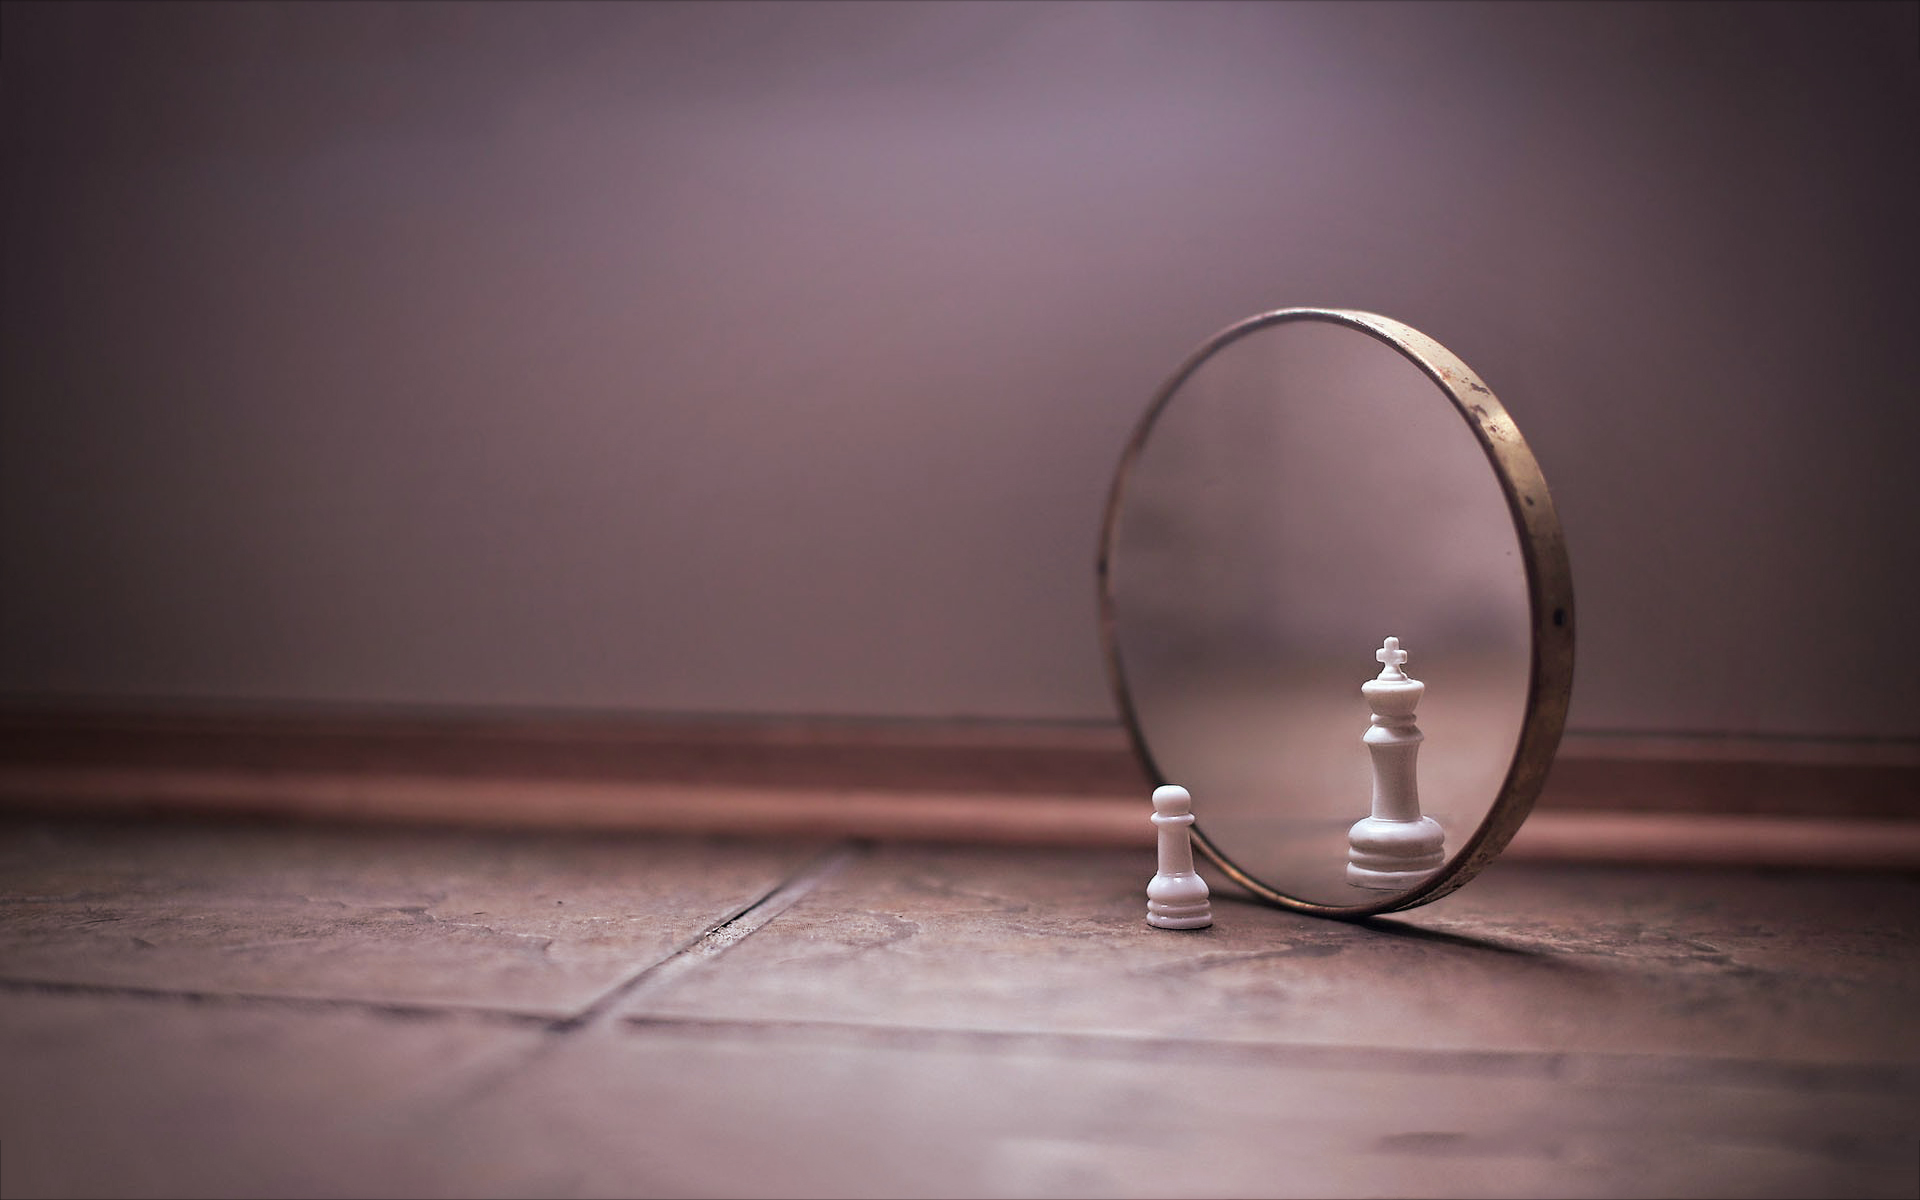
\includegraphics[height=\paperheight]{../img/cover_background.jpg}
    }
    \maketitle
  }

%%%%%%%%%%%%%%%%%%%%%%%%%%%%%%%%%%%%%%%%%%%%%%%%%%%%%%%%%%%%%%%%%%%%%%%%%%%%%%%%

  \section{The Alpha* Timeline}
  {
    \setbeamertemplate{frame footer}{\url{https://en.wikipedia.org/wiki/Fan_Hui}}
    \begin{frame}{Fan Hui}
      \begin{center}
        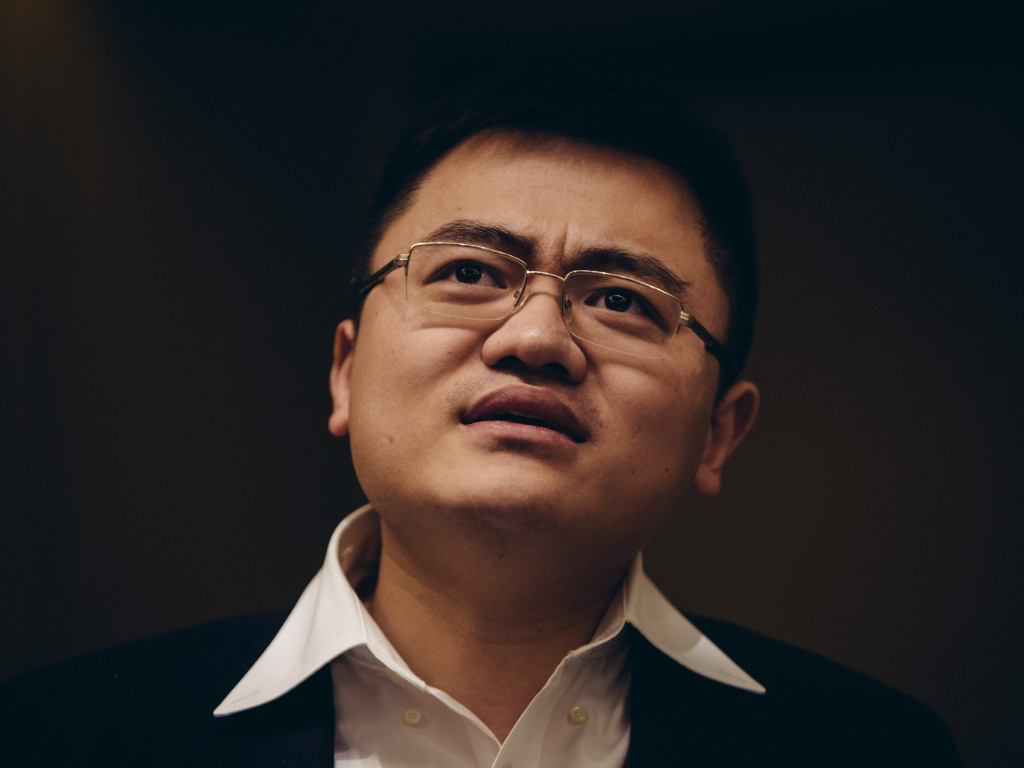
\includegraphics[width=.55\textwidth]{../img/Fan_Hui_profile.jpg}
      \end{center}
      \pause
      \vskip -1.6em
      \begin{itemize}[<+- | alert@+>]
        \item professional 2 dan
        \item European Go Champion in 2013, 2014 and 2015
        \item European Professional Go Champion in 2016 
      \end{itemize}
    \end{frame}
  }

  \begin{frame}{AlphaGo vs. Fan Hui}
    \pause
    \begin{center}
      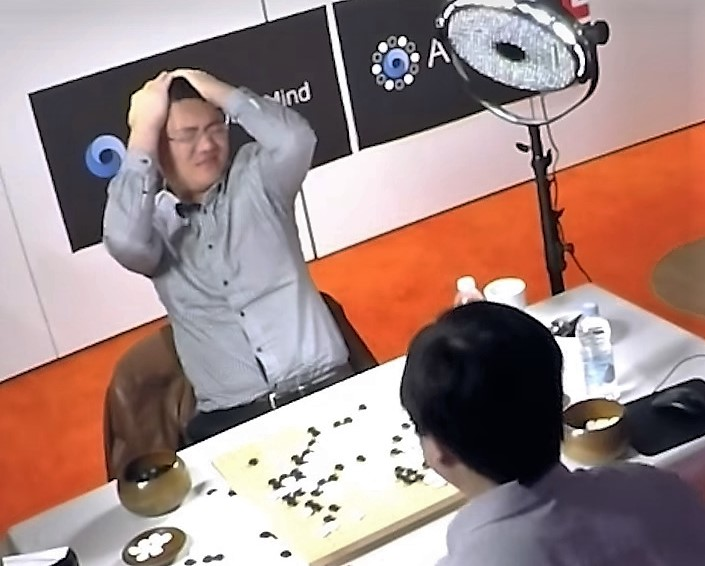
\includegraphics[width=.55\textwidth]{../img/Fan_Hui_loses.jpg}
    \end{center}
    \textbf{AlphaGo won 5:0} in a~formal match on~October 2015.
    \pause

    \vskip -1em
    \epigraph{
      \tiny
      [AlphaGo] is very strong and stable, it seems like a~wall.
      ...
      I know AlphaGo is a~computer, but if no one told me, maybe I would think the player was a~little strange, but a~very strong player, a~real person.
    }{Fan Hui}
  \end{frame}

  {
    \setbeamertemplate{frame footer}{\url{https://en.wikipedia.org/wiki/Lee_Sedol}}
    \begin{frame}{Lee Sedol ``The Strong Stone''}
      \begin{center}
        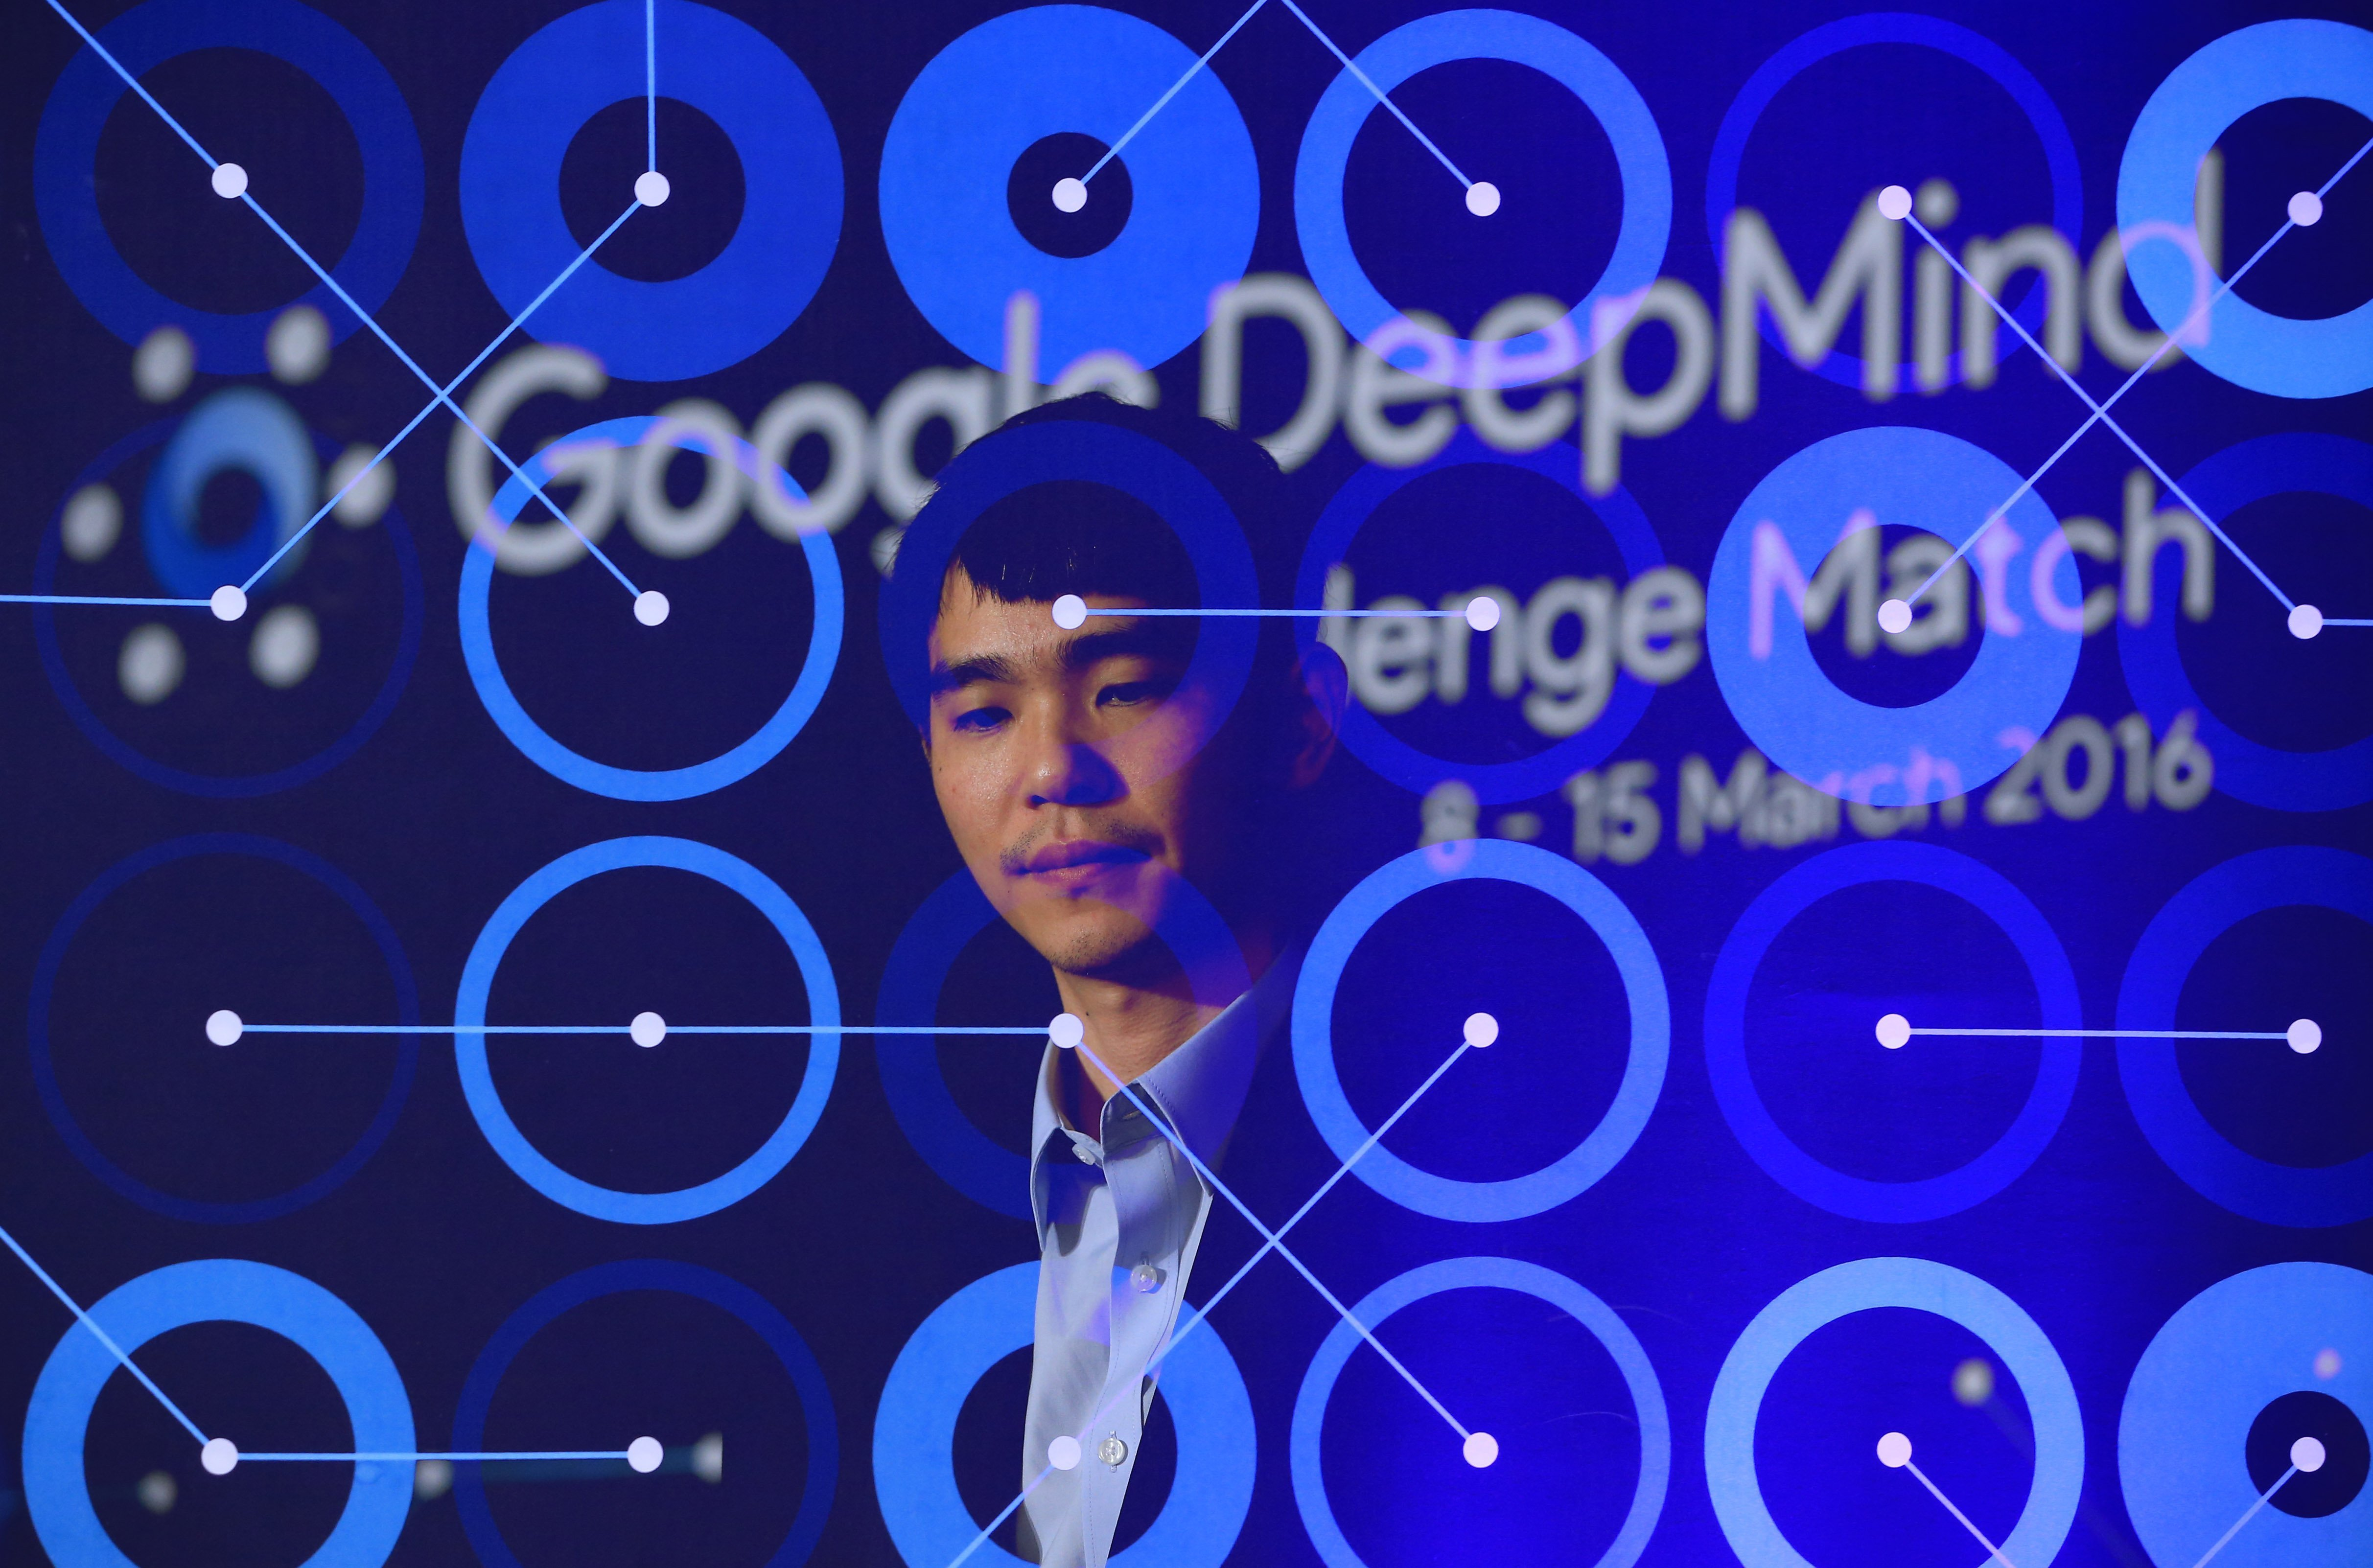
\includegraphics[width=.55\textwidth]{../img/Lee_Sedol_profile_2.jpg}
      \end{center}
      \pause
      \vskip -1.6em
      \begin{itemize}[<+- | alert@+>]
        \item professional 9 dan 
        \item the $2^{nd}$ in international titles
        \item the $5^{th}$ youngest to become a~professional Go player in~South Korean history
        \item Lee Sedol would win 97 out of~100 games against Fan Hui.
        \item ``Roger Federer'' of~Go
      \end{itemize}
    \end{frame}
  }

  {
    \usebackgroundtemplate{
      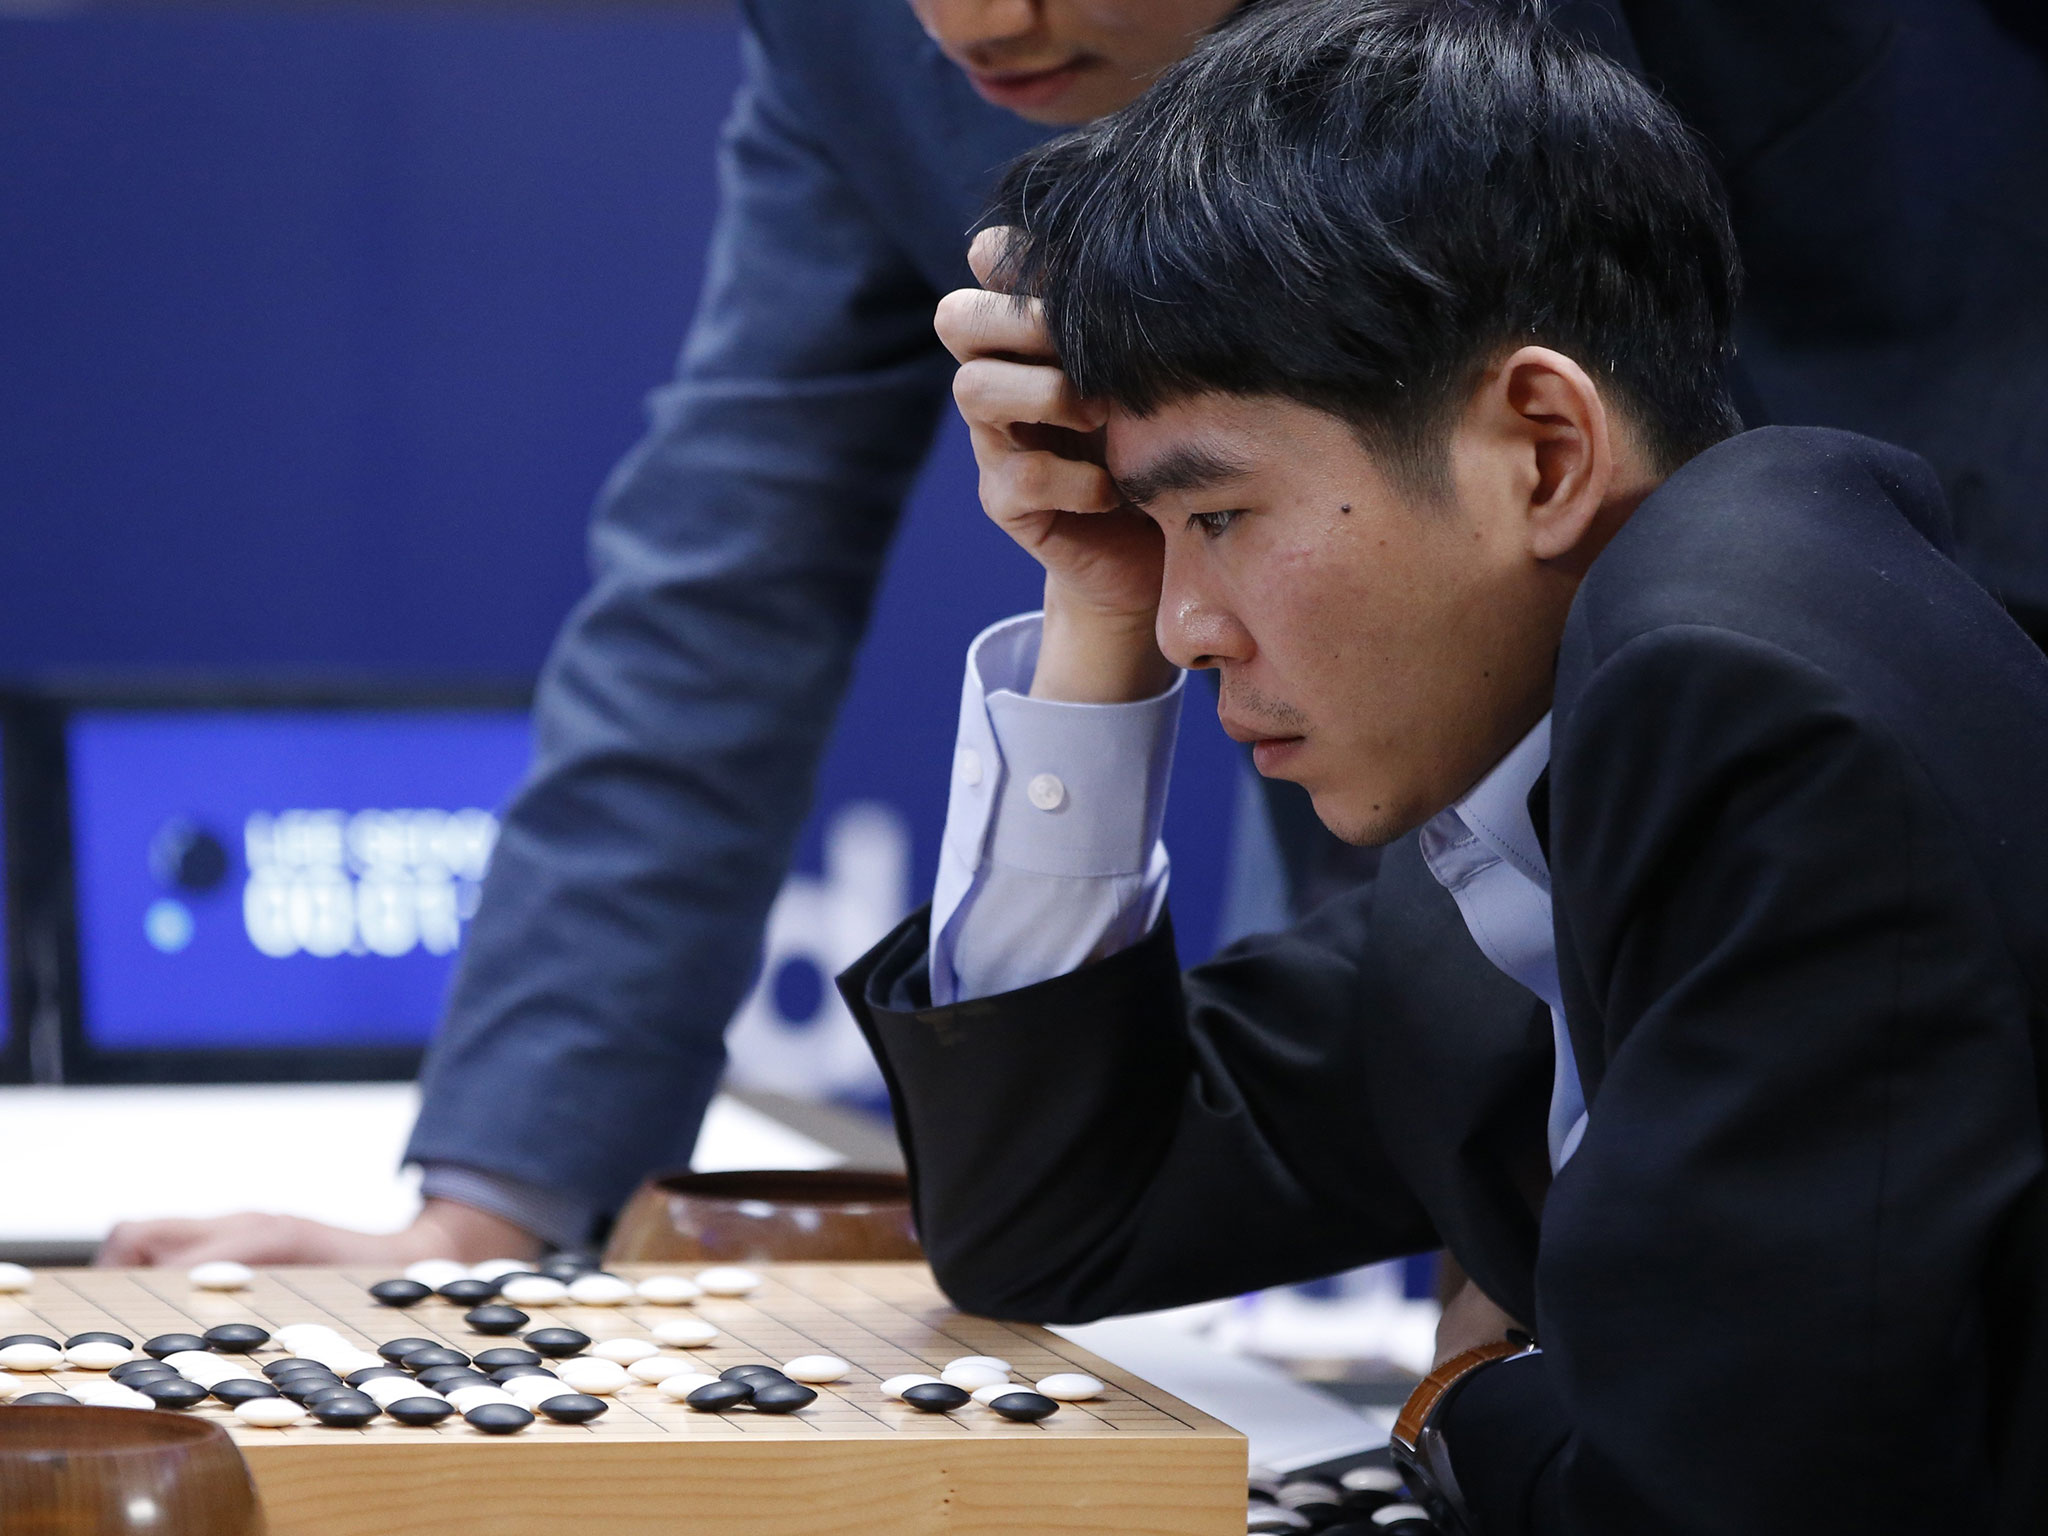
\includegraphics[height=\paperheight]{../img/Lee_Sedol_quotes.jpg}
    }
    \begin{frame}[standout]
      \epigraph{
        \tiny
        I heard Google DeepMind's AI is surprisingly strong and getting stronger, but I am confident that I can win, at least this time.
      }{Lee Sedol}
      \pause

      \epigraph{
        \tiny
        ...even beating AlphaGo by 4:1 may allow the Google DeepMind team to claim its de facto victory and the defeat of him [Lee~Sedol], or even humankind.
      }{interview in JTBC Newsroom}
      \pause
    \end{frame}
  }

  {
    \usebackgroundtemplate{
      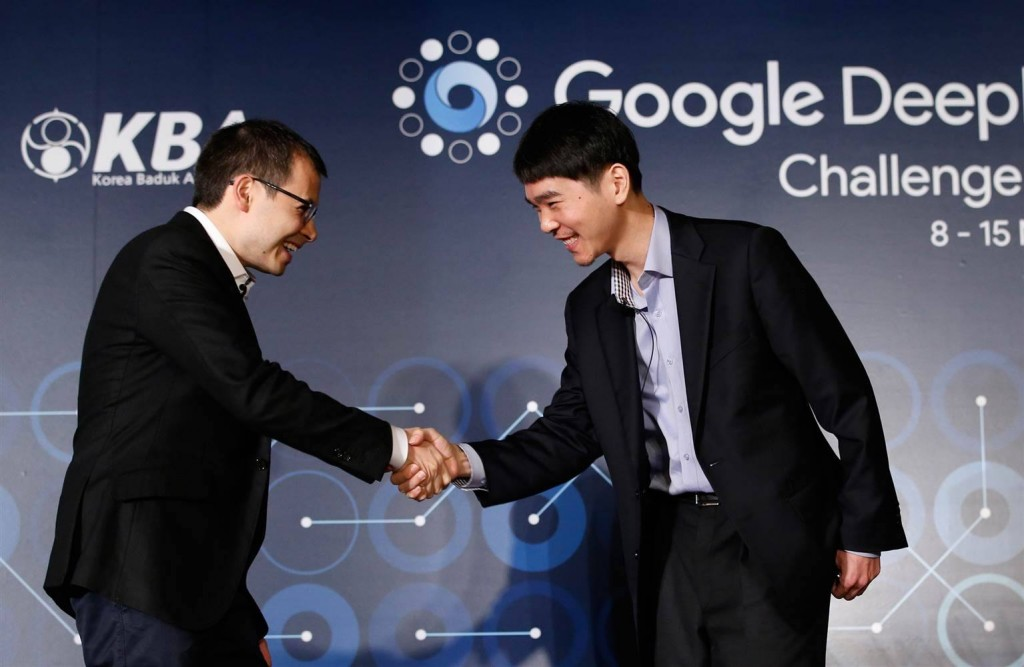
\includegraphics[height=\paperheight]{../img/Lee_Sedol_after_match.jpg}
    }
    \setbeamertemplate{frame footer}{\color{white}\url{https://en.wikipedia.org/wiki/AlphaGo_versus_Lee_Sedol}}
    \begin{frame}{AlphaGo vs. Lee Sedol}
      \pause

      \vskip 1em
      \color{white}
      In March 2016 \textbf{AlphaGo won 4:1} against the legendary Lee Sedol.
      \pause

      AlphaGo won all but the $4^{th}$ game; all games were won by~resignation.
      \pause
    \end{frame}
  }

  {
    \usebackgroundtemplate{
      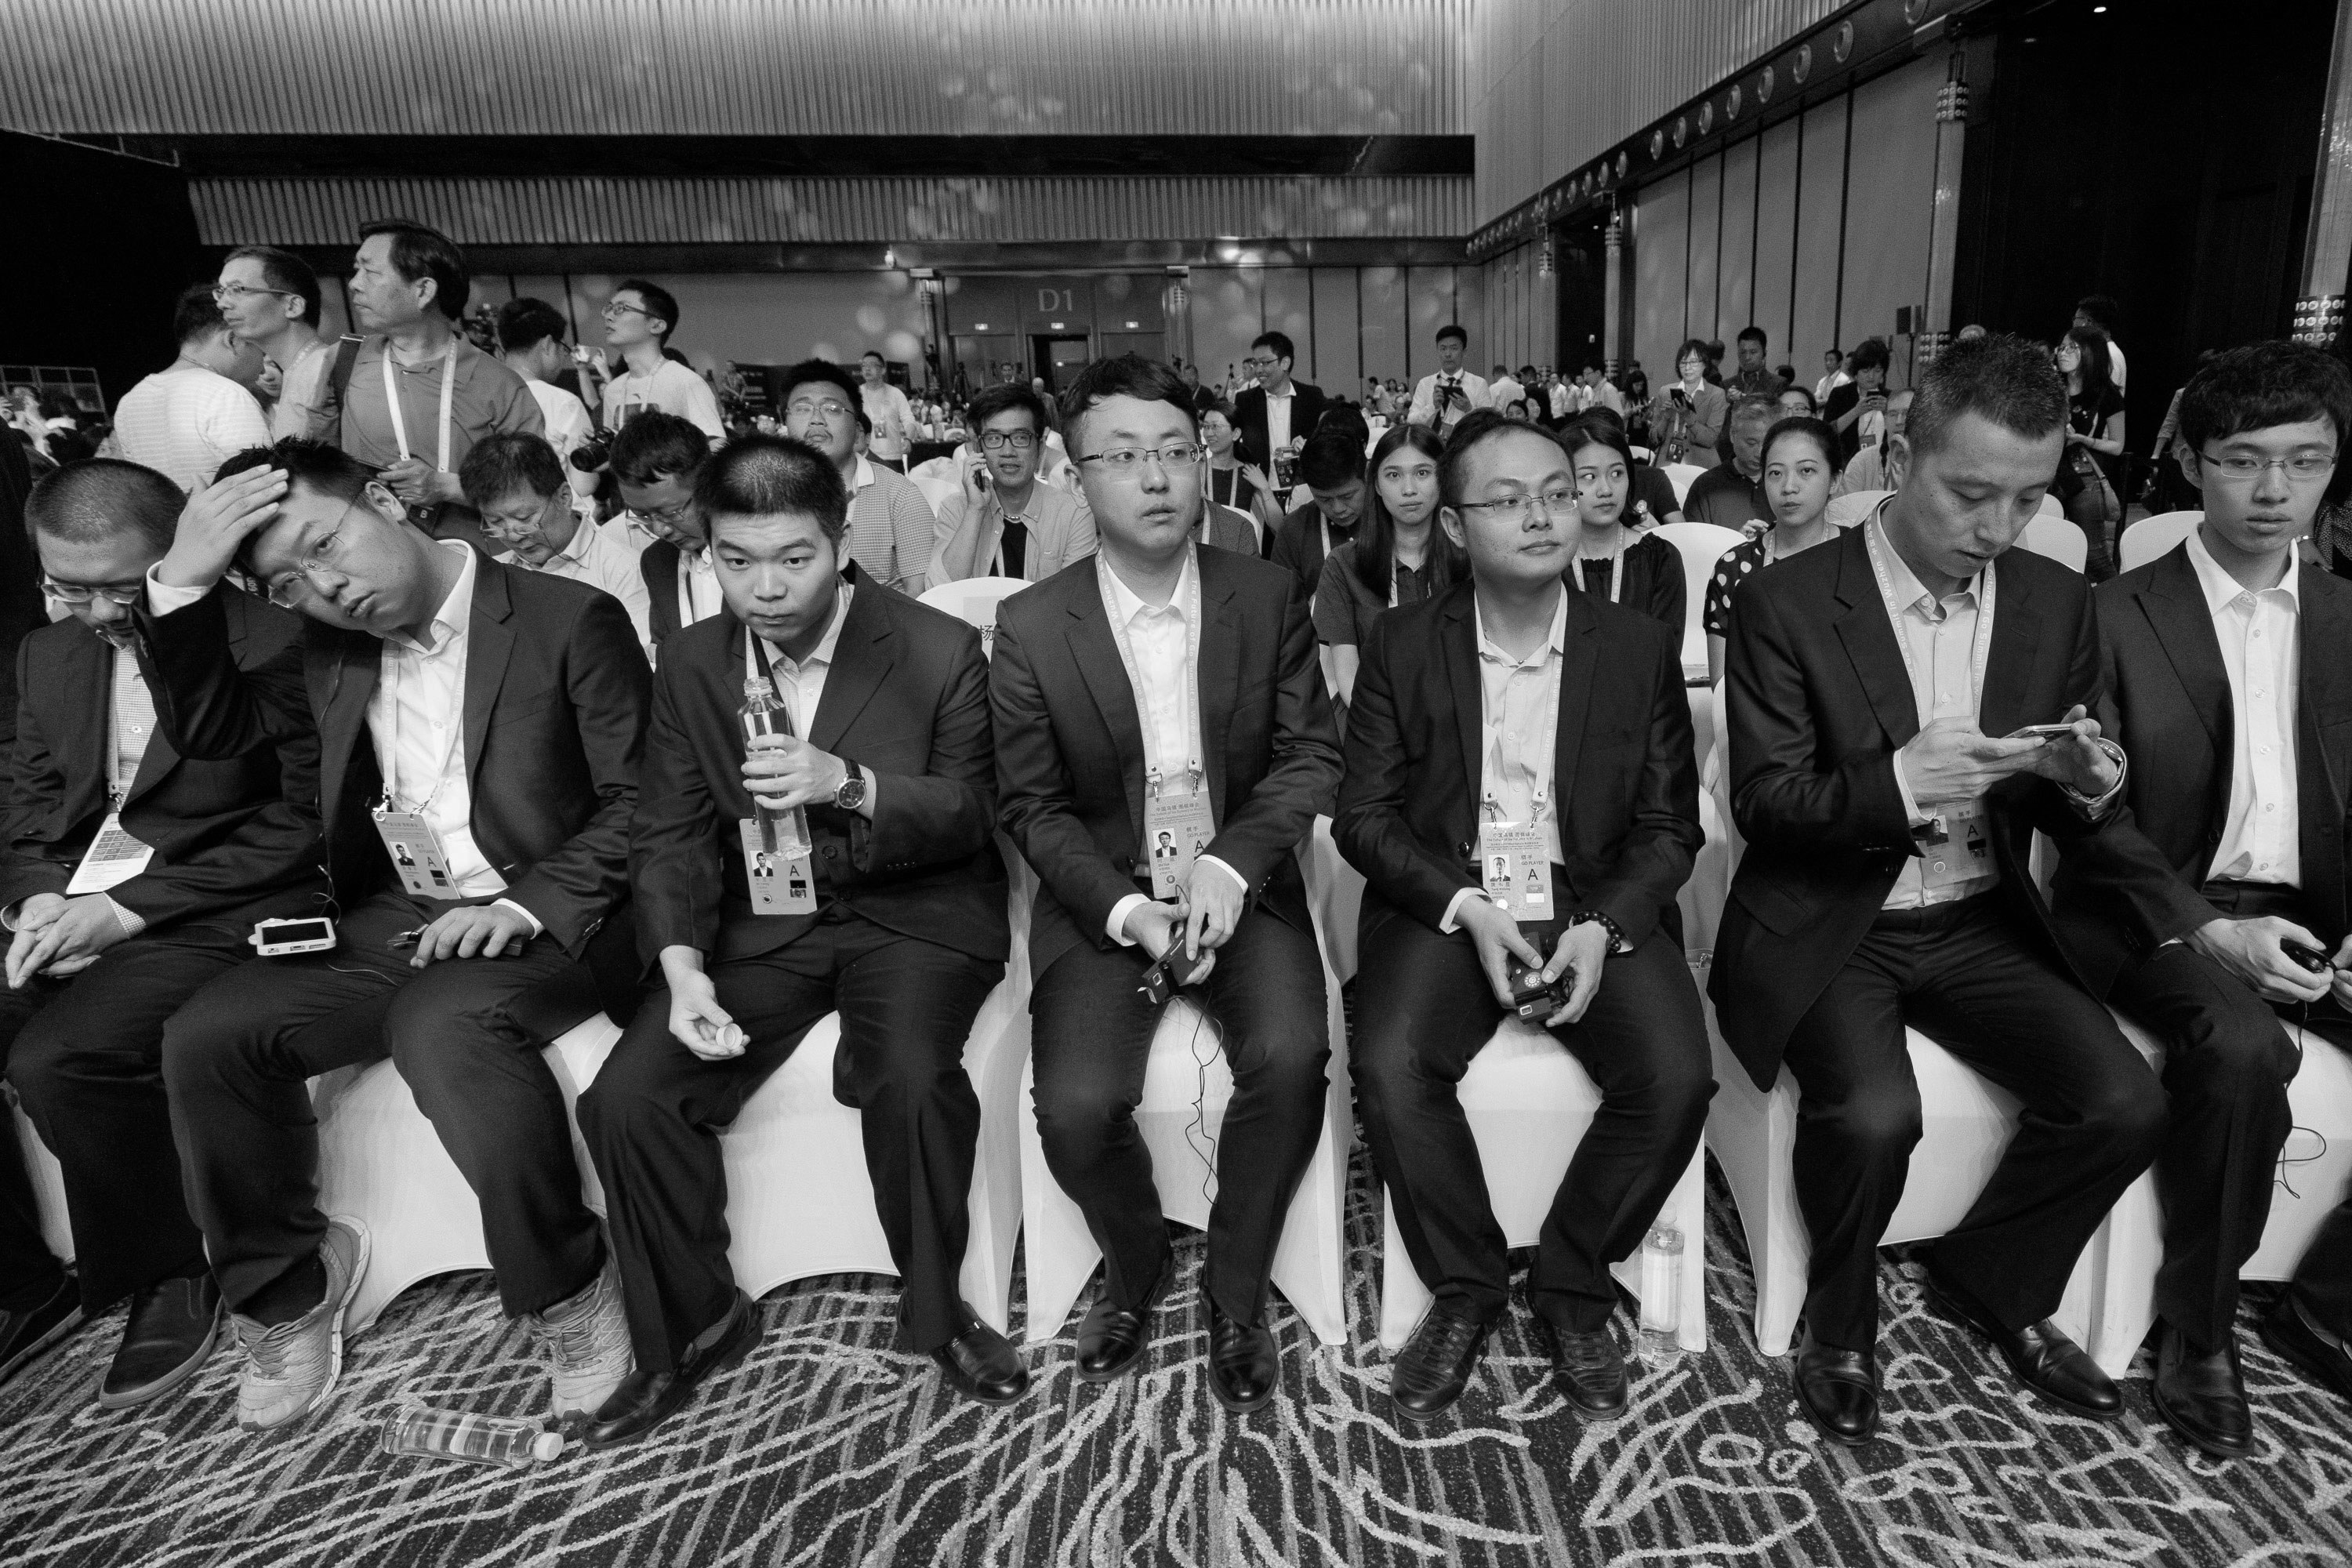
\includegraphics[height=\paperheight]{../img/Go_masters_grayscale.jpg}
    }
    \setbeamertemplate{frame footer}{\color{white}\url{https://deepmind.com/research/alphago/match-archive/master/}}
    \begin{frame}{AlphaGo Master}
      \pause

      \color{white}
      In January 2017, DeepMind revealed that AlphaGo had played a~series of~unofficial online games against some of~the strongest professional Go players under the pseudonyms ``Master'' and ''Magister''.
      \pause

      This AlphaGo was an~improved version of~the AlphaGo that played Lee Sedol in~2016.
      \pause

      Over one week, AlphaGo played 60 online fast time-control games.
      \pause

      \textbf{AlphaGo won this series of games 60:0.}
    \end{frame}
  }

  {
    \setbeamertemplate{frame footer}{\color{black}\url{https://events.google.com/alphago2017/}}

    \usebackgroundtemplate{
      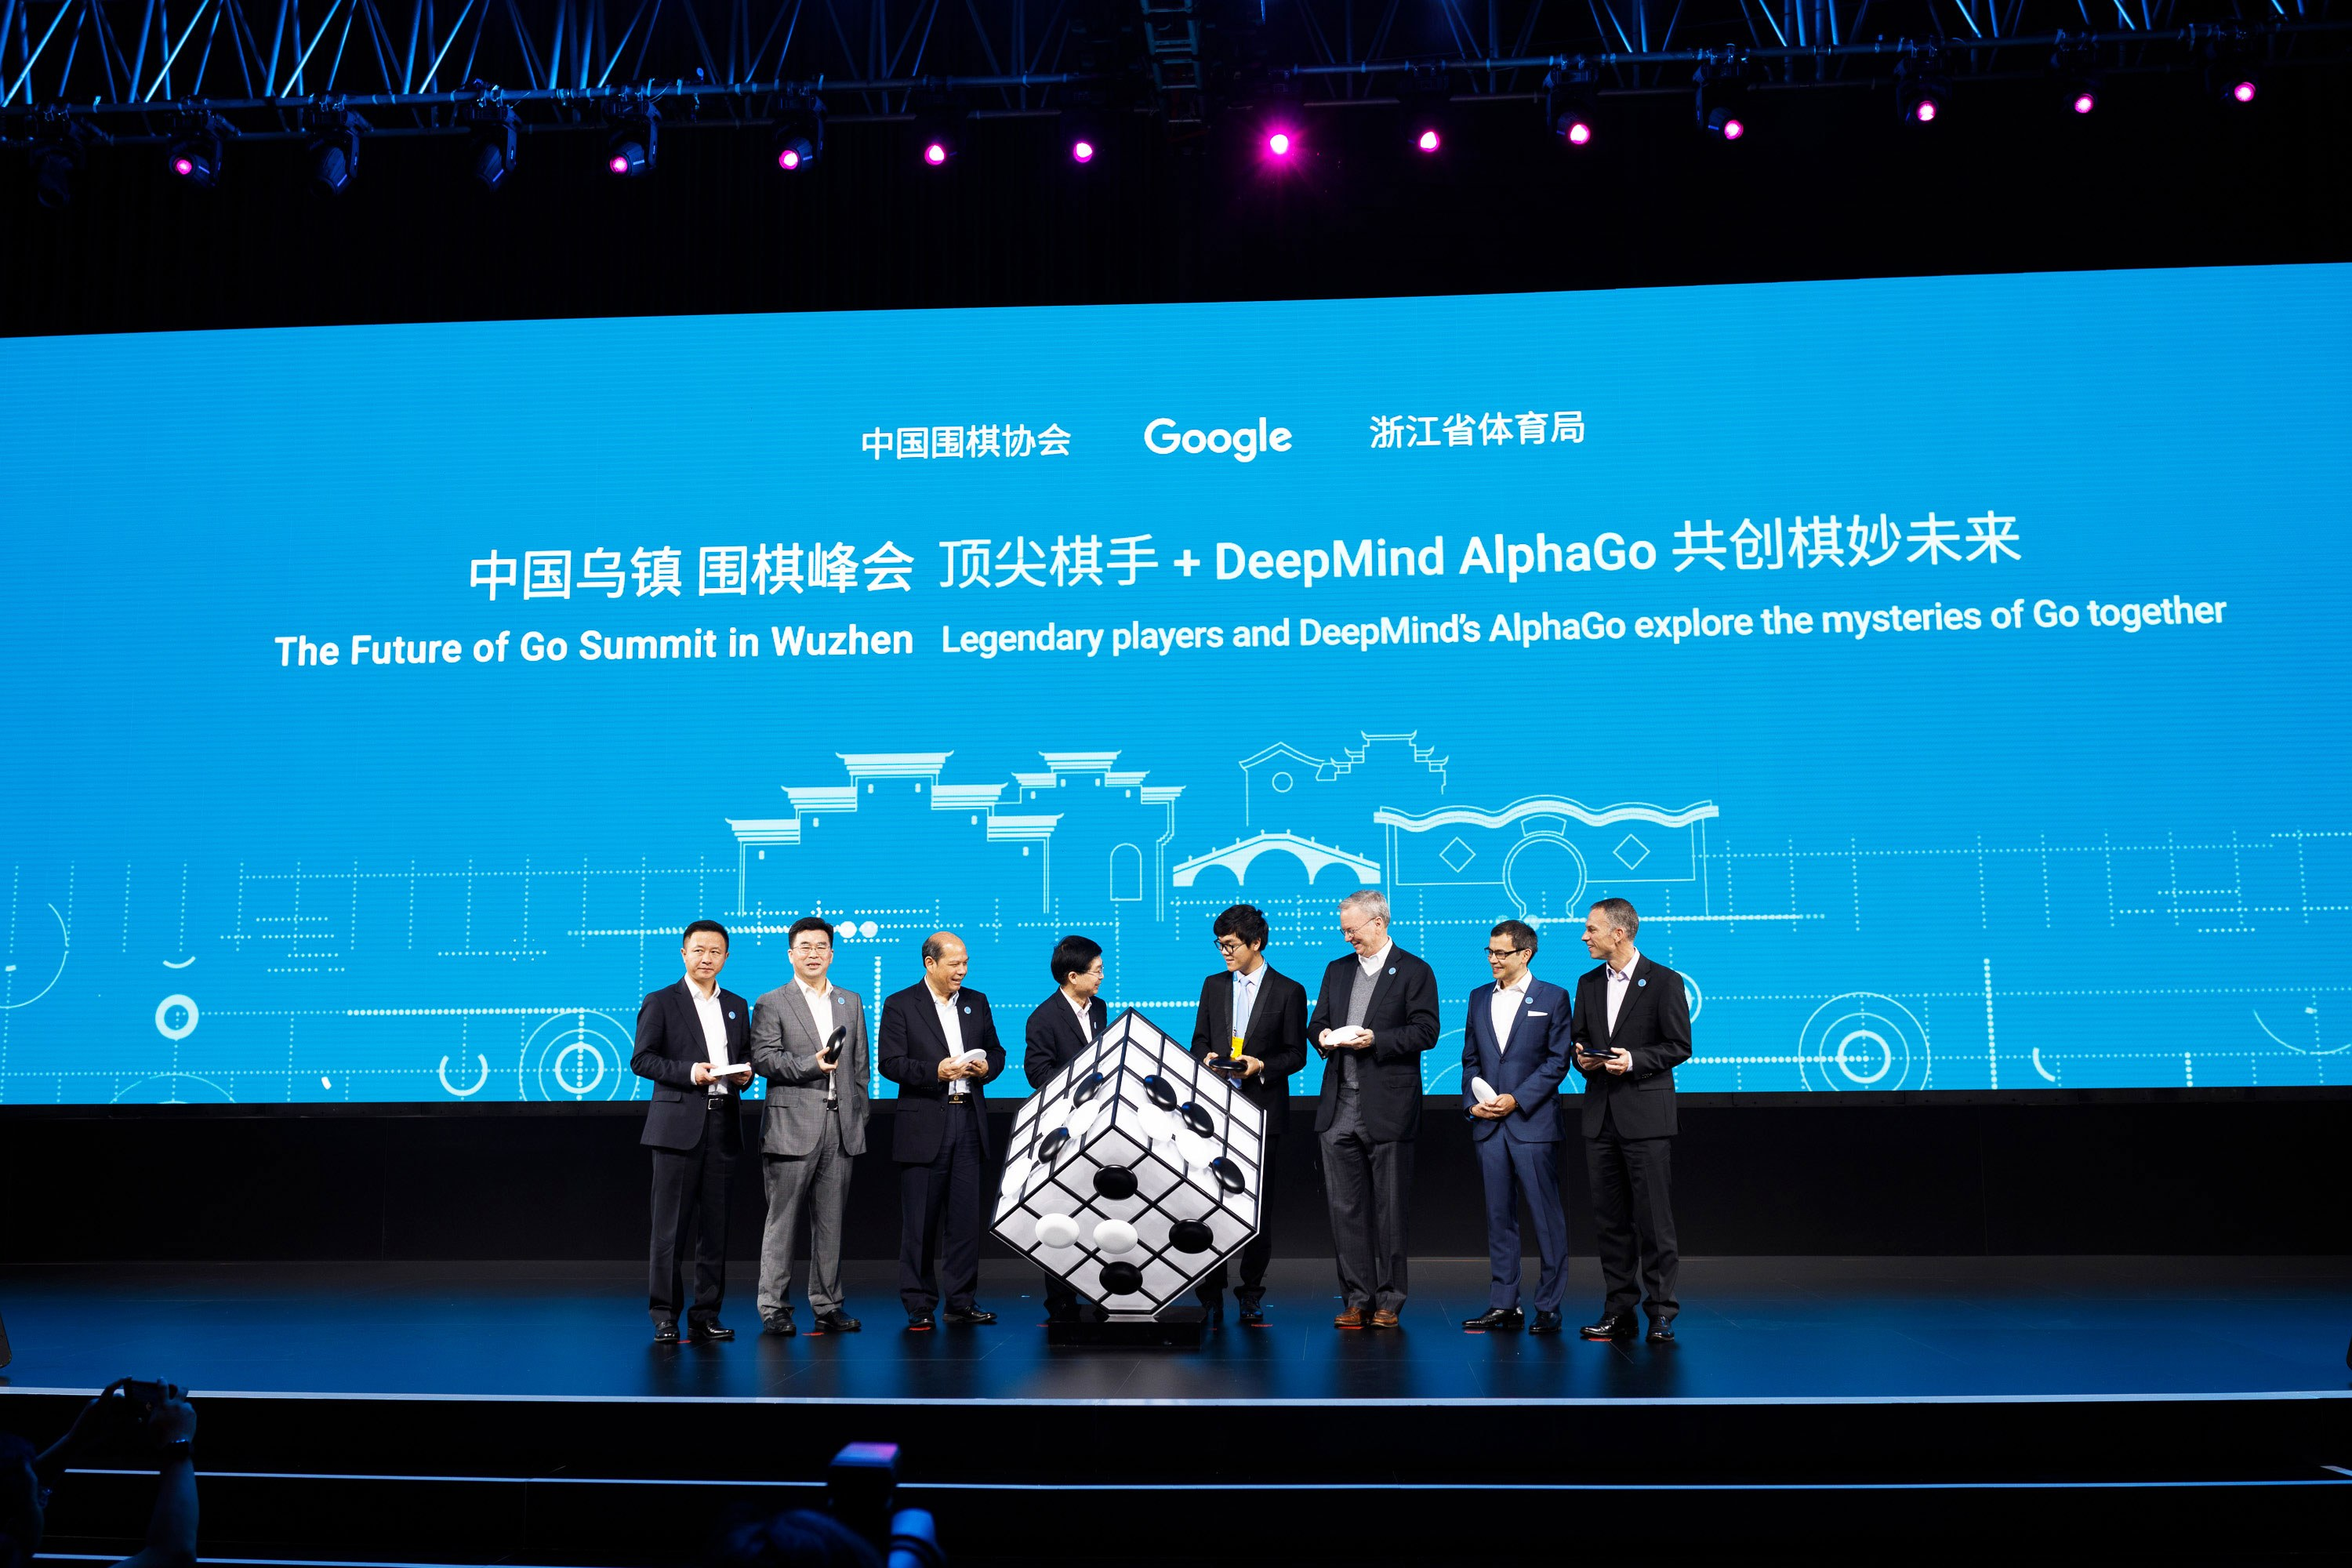
\includegraphics[height=\paperheight]{../img/future_of_Go_summit.jpg}
    }
    \begin{frame}[standout]
    \end{frame}

    \usebackgroundtemplate{
      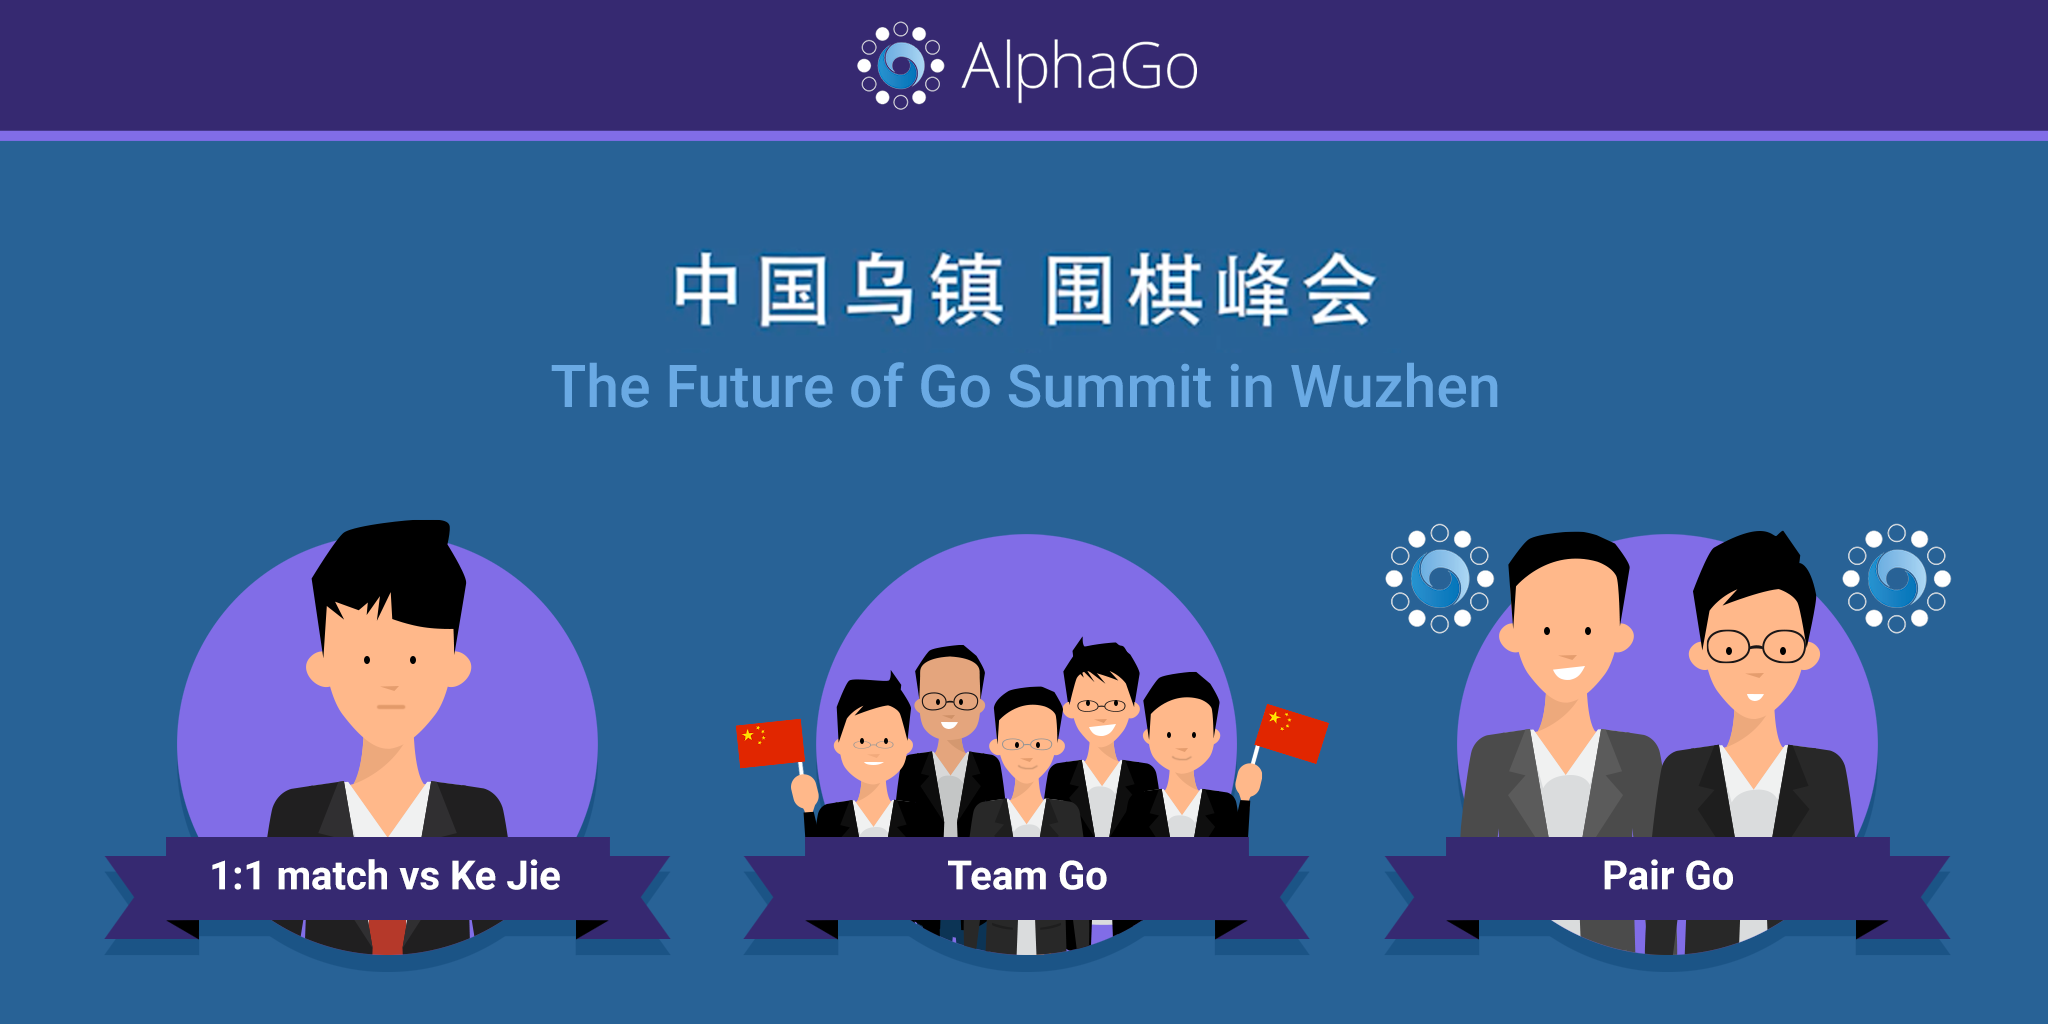
\includegraphics[width=\paperwidth]{../img/future_of_Go_summit_infographics.jpg}
    }
    \begin{frame}
      \vskip .7\textheight

      \pause
      \begin{itemize}[<+- | alert@+>]
        \item 23 May - 27 May 2017 in Wuzhen, China
        \item Team Go vs. AlphaGo \textbf{0:1}
        \item AlphaGo vs. world champion Ke Jie \textbf{3:0}
      \end{itemize}
    \end{frame}
  }

  {
    \usebackgroundtemplate{
      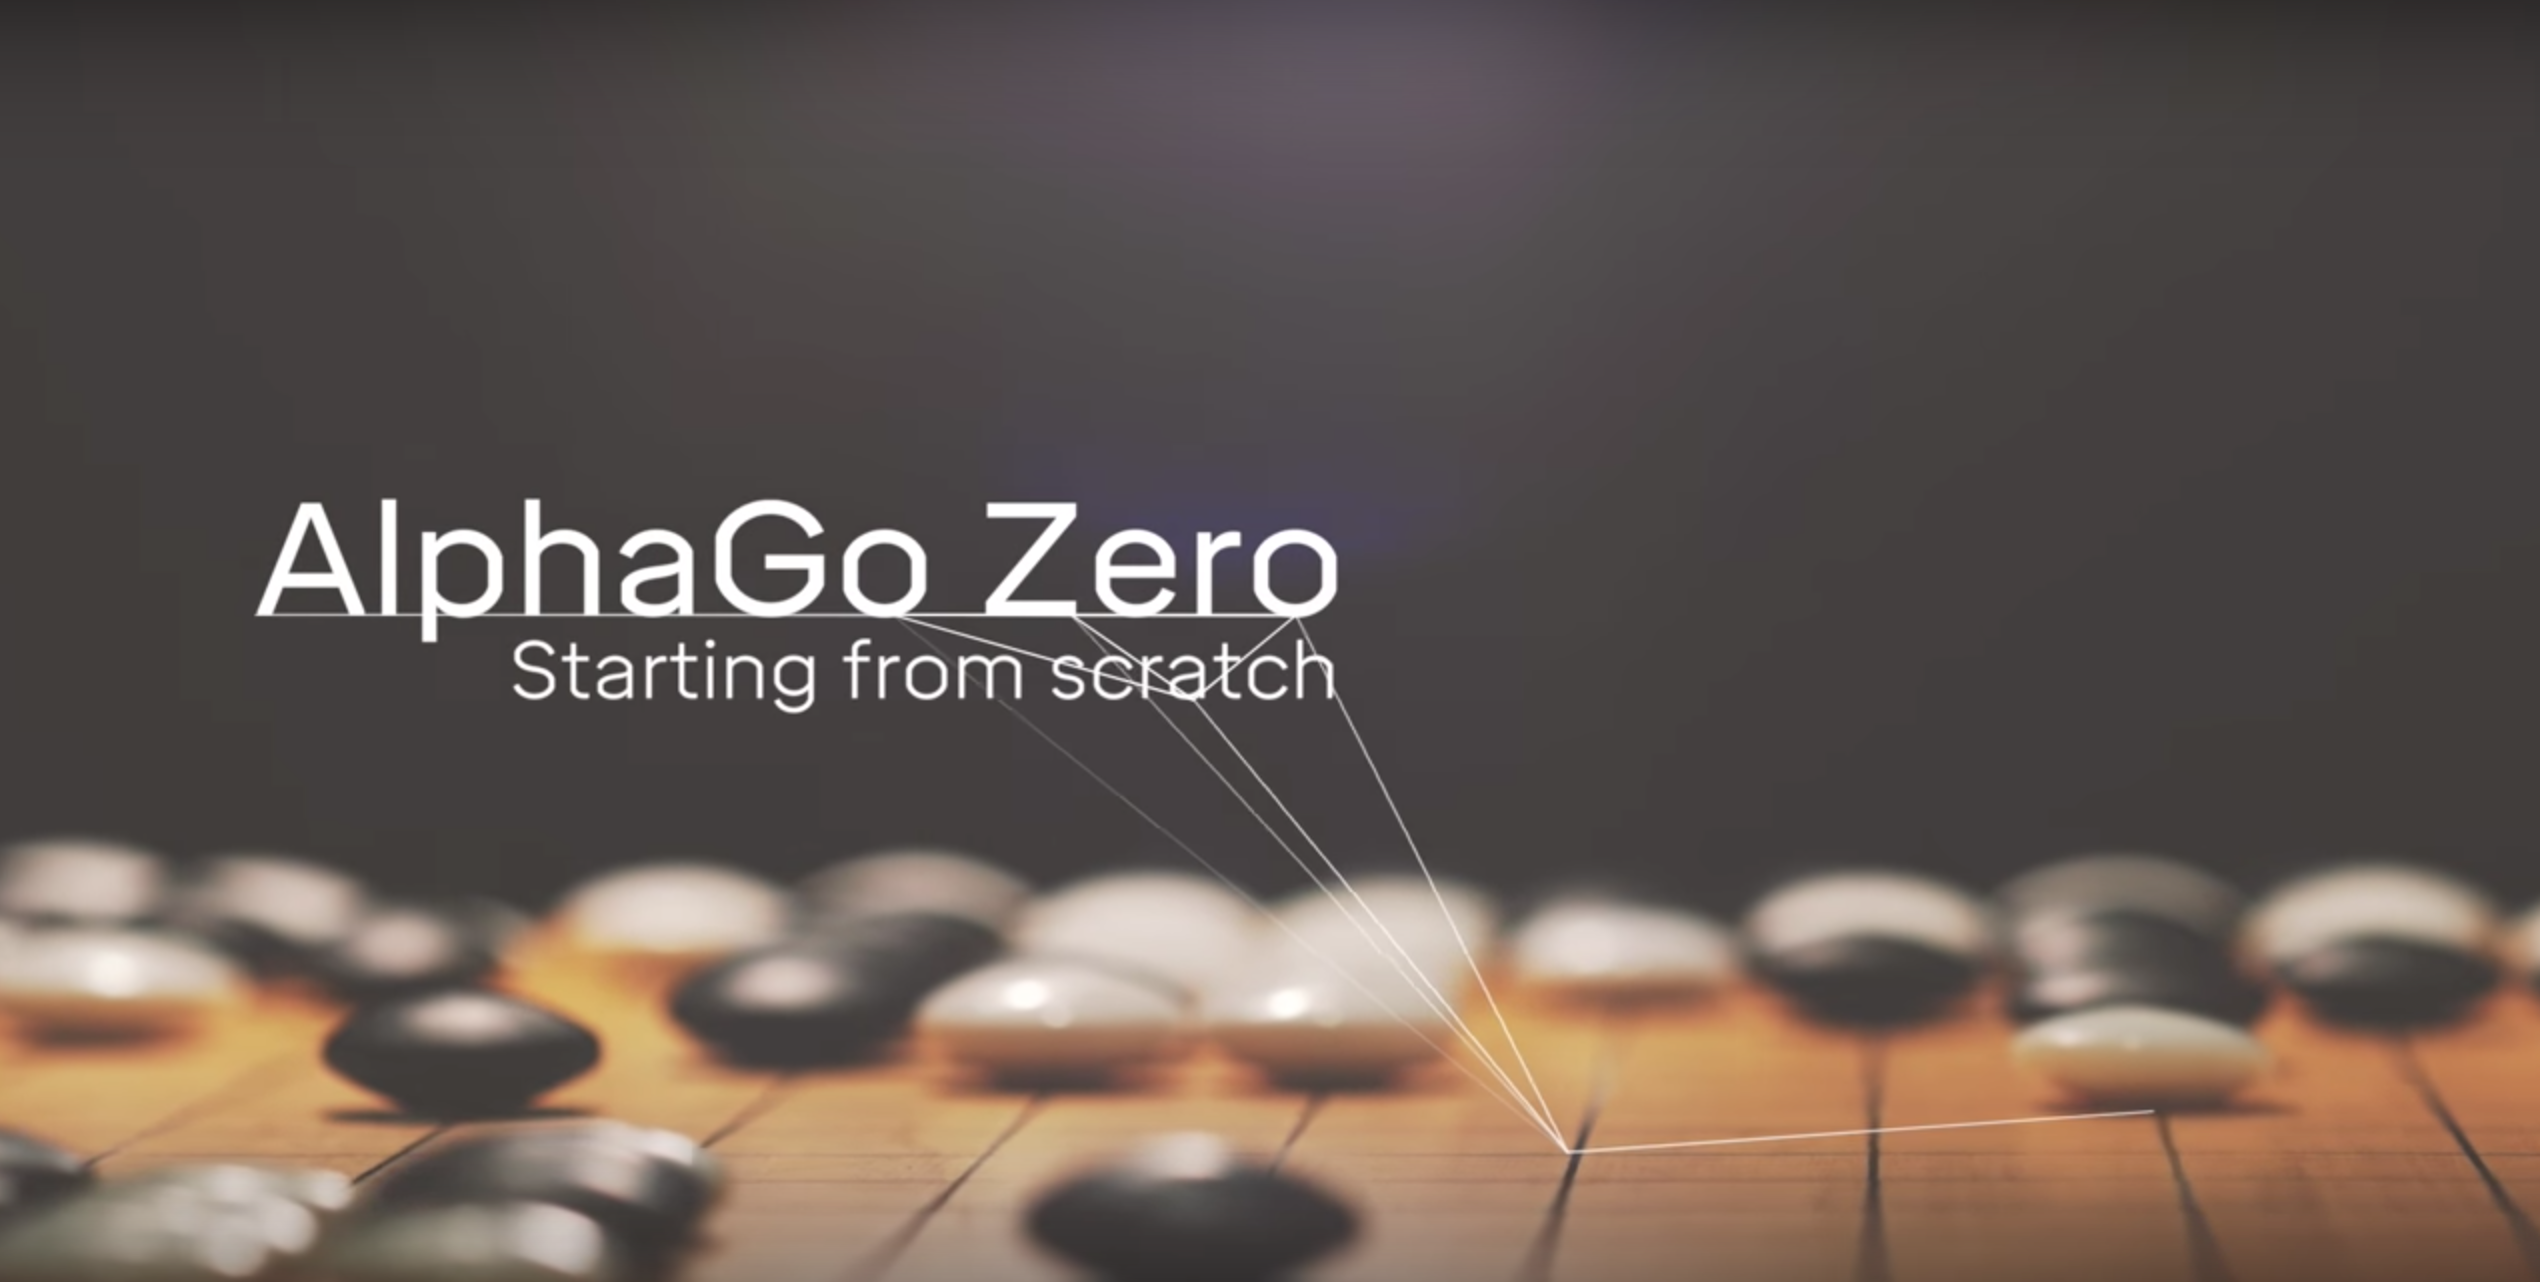
\includegraphics[height=\paperheight]{../img/AlphaGo_Zero.png}
    }
    \begin{frame}[standout]
      \pause
      \vskip .4\textheight
      defeated AlphaGo Lee by \alert{100 games to 0}
    \end{frame}
  }

  {
    \usebackgroundtemplate{
      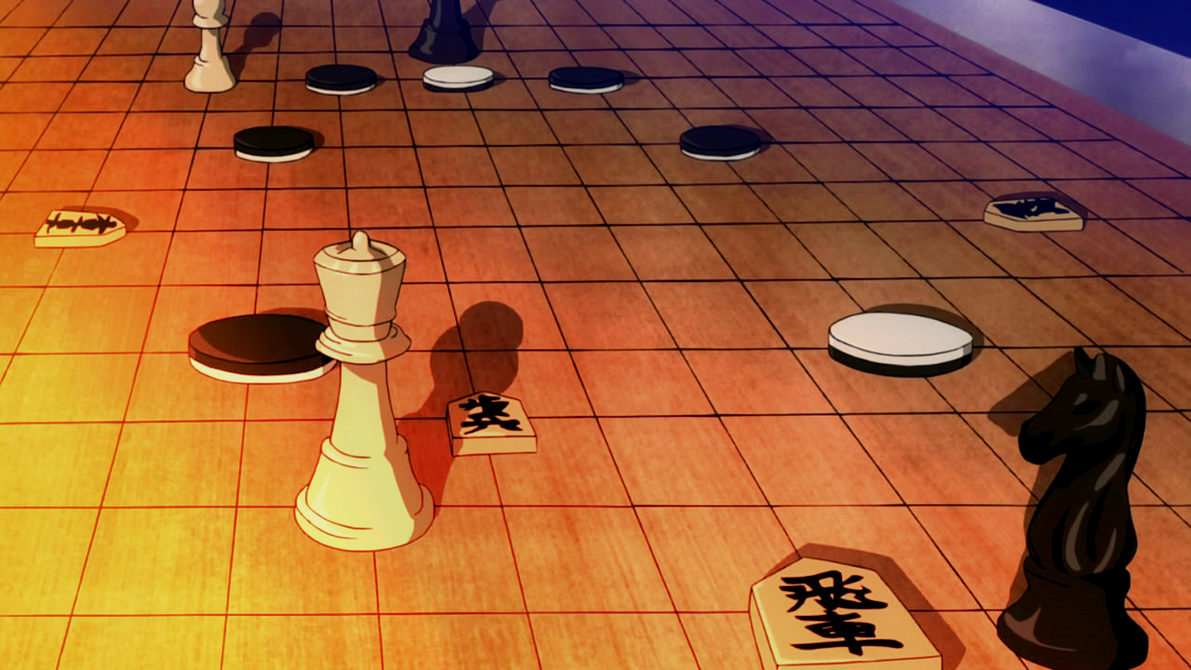
\includegraphics[height=\paperheight]{../img/chess-go-shogi.png}
    }
    \begin{frame}
      \color{black}
      \epigraph{
        \alert{AI system that mastered chess, Shogi and Go to ``superhuman levels'' within a~handful of~hours}
      }{\Huge AlphaZero}
      \pause
      \vskip 1em
      defeated AlphaGo Zero (version with 20 blocks trained for 3 days) by~\textbf{60 games to 40}
    \end{frame}
  }

  {
    \usebackgroundtemplate{
      
\includegraphics[height=\paperheight]{../img/deepmind.png}
    }
    \setbeamertemplate{enumerate items}[circle]{\color{white}}
    \begin{frame}[standout]
      \pause
      \begin{enumerate}[<+- | alert@+>]
        \item AlphaGo Fan
        \item AlphaGo Lee
        \item AlphaGo Master
        \item AlphaGo Zero
        \item AlphaZero
      \end{enumerate}
    \end{frame}
  }

%%%%%%%%%%%%%%%%%%%%%%%%%%%%%%%%%%%%%%%%%%%%%%%%%%%%%%%%%%%%%%%%%%%%%%%%%%%%%%%%

  \section{AlphaGo}
  {
    \setbeamertemplate{frame footer}{[\cite{Silver2016mastering}]}

    \begin{frame}{Policy and Value Networks}
      \begin{center}
        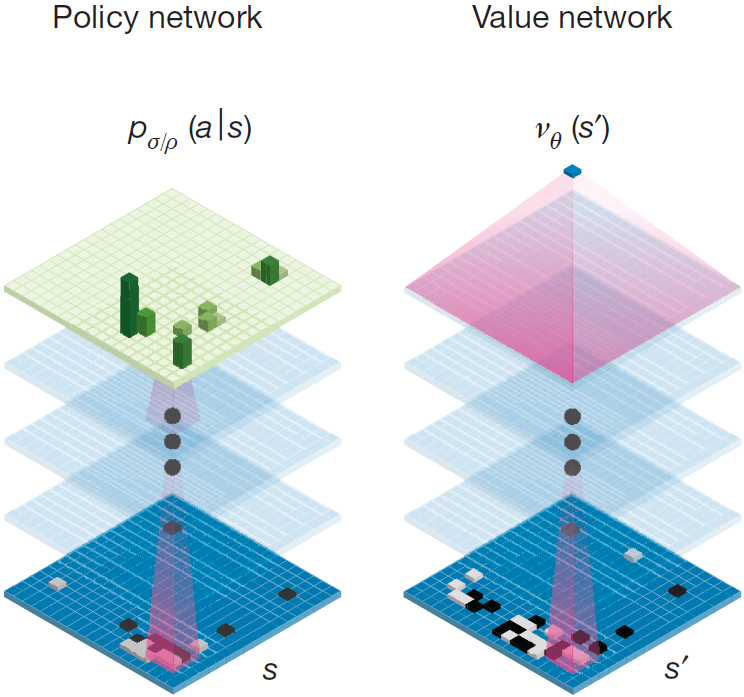
\includegraphics[height=.85\textheight]{../img/policy_and_value_network.png}
      \end{center}
    \end{frame}

    \begin{frame}{Training the (Deep Convolutional) Neural Networks}
      \begin{center}
        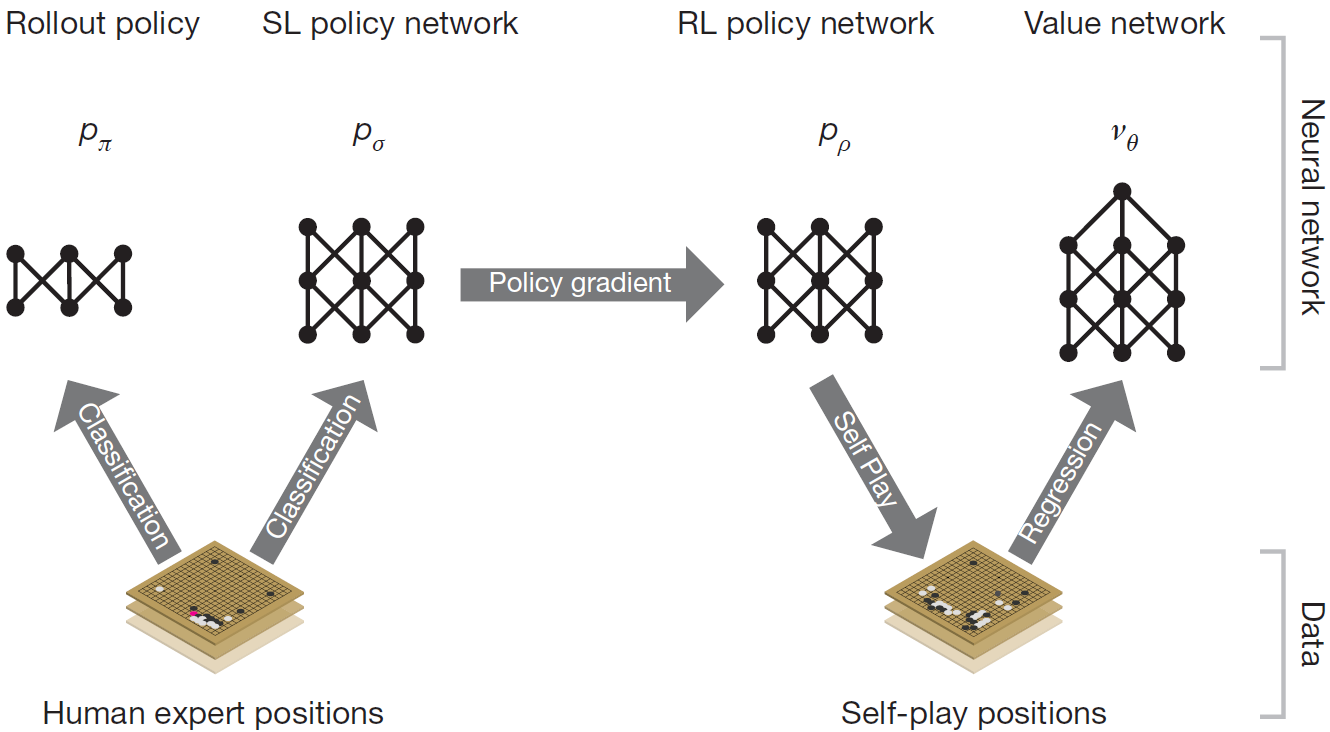
\includegraphics[width=\textwidth]{../img/neural_nets_pipeline.png}
      \end{center}
    \end{frame}
  }

%%%%%%%%%%%%%%%%%%%%%%%%%%%%%%%%%%%%%%%%%%%%%%%%%%%%%%%%%%%%%%%%%%%%%%%%%%%%%%%%

  \section{AlphaGo Zero (AG0)}
  {
    \setbeamertemplate{frame footer}{[\cite{Silver2017AlphaGoZero}]}

    \begin{frame}{AG0: Differences Compared to AlphaGo \{Fan, Lee, Master\}}
      AlphaGo \{Fan, Lee, Master\} $\times$ \alert{AlphaGo Zero}:
      \pause
      \begin{itemize}[<+->]
        \item supervised learning from human expert positions $\times$ \alert{from scratch by self-play reinforcement learning (``tabula rasa'')}
        \item additional (auxialiary) input features $\times$ \alert{only the black and white stones from the board as input features}
        \item separate policy and value networks $\times$ \alert{single neural network}
        \item tree search using also Monte Carlo rollouts $\times$ \alert{simpler tree search using only the single neural network to both evaluate positions and sample moves}
        \item distributed machines + 48 tensor processing units (TPUs) (AlphaGo Lee) $\times$ \alert{single machines + 4 TPUs}
        \item several months of~training time (AlphaGo Lee) $\times$ \alert{72 h of training time (outperforming AGLee after 36 h)}
      \end{itemize}
      \pause

      AG0 achieves this via
      \begin{itemize}[<+->]
        \item a~new \alert{reinforcement learning} algorithm
        \item with \alert{lookahead search inside the training loop}
      \end{itemize}
    \end{frame}

    \begin{frame}{AG0: Self-Play Reinforcement Learning}
      \pause
      \begin{center}
        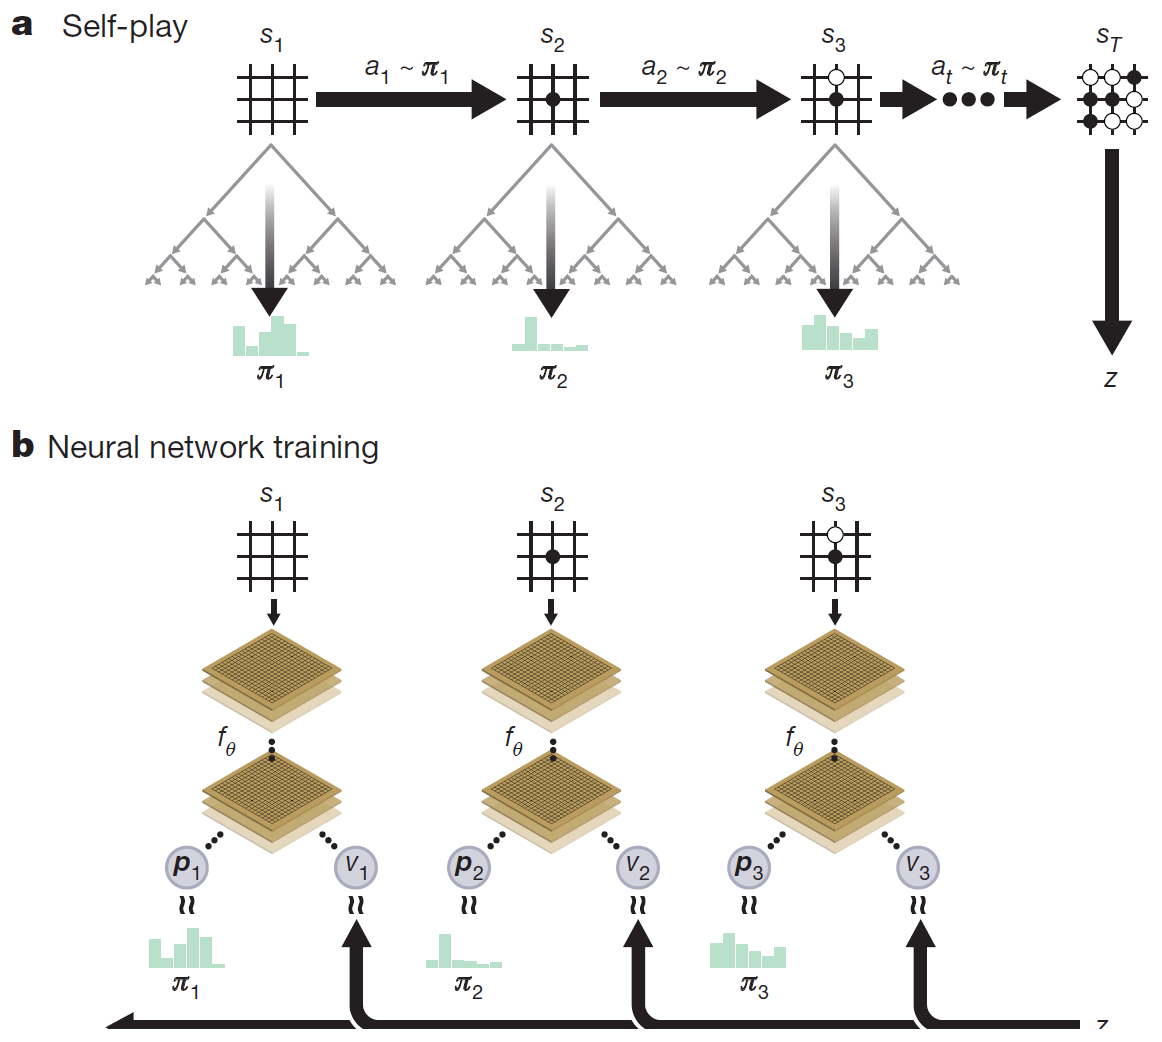
\includegraphics[height=.9\textheight]{../img/AG0-paper/self-play-RL-in-AG0.png}
      \end{center}
    \end{frame}

    \begin{frame}{AG0: Self-Play Reinforcement Learning -- Neural Network}
      deep neural network $f_\theta$ with parameters~$\theta$:
      \pause
      \begin{itemize}[<+- | alert@+>]
        \item input: raw board representation~$s$
        \item output:
          \begin{itemize}[<+- | alert@+>]
            \item move probabilities $\p$
            \item value $v$ of~the board position
            \item $f_\theta(s) = (\p, v)$
          \end{itemize}
        \item specifics:
          \begin{itemize}[<+- | alert@+>]
            \item (20 or 40) residual blocks (of convolutional layers)
            \item batch normalization
            \item rectifier non-linearities
          \end{itemize}
      \end{itemize}
    \end{frame}

    \begin{frame}{AG0: Comparison of Various Neural Network Architectures}
      \begin{center}
        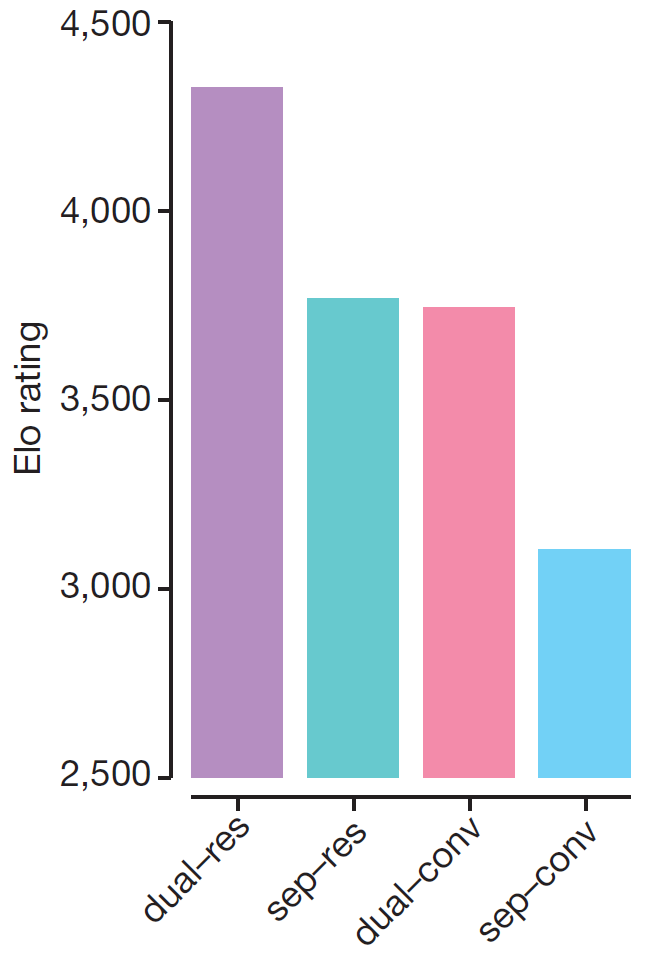
\includegraphics[height=.9\textheight]{../img/AG0-paper/nn-arch-vs-elo.png}
      \end{center}
    \end{frame}

    \begin{frame}{AG0: Self-Play Reinforcement Learning -- Steps}
      \begin{enumerate}[<+- | alert@+>]
        \item[0.] random weights $\theta_0$
        \item at each iteration $i > 0$, self-play games are generated:
          \begin{enumerate}[<+- | alert@+>]
            \item[i.] MCTS samples search probabilities $\mathbf{\pi}_t$ based on the neural network from the previous iteration $f_{\theta_{i-1}}$:
              $$\mathbf{\pi}_t = \alpha_{\theta_{i-1}}(s_t)$$
              for each time-step $t = 1, 2, \ldots, T$
            \item[ii.] move is sampled from $\mathbf{\pi}_t$
            \item[iii.] data $(s_t, \mathbf{\pi}_t, z_t)$ for each $t$ are stored for later training
            \item[iv.] new neural network $f_{\theta_{i}}$ is trained in order to minimize the loss
              $$l = (z - v)^2 - \mathbf{\pi}^\top \log \p + c || \theta ||^2$$
          \end{enumerate}
      \end{enumerate}
      \pause
      \vskip -2em
      Loss~$l$ makes $(\p, v) = f_\theta(s)$ more closely match the improved search probabilities and self-play winner $(\mathbf{\pi}, z)$.
    \end{frame}

    \begin{frame}{AG0: Monte Carlo Tree Search (1/2)}
      Monte Carlo Tree Search (MCTS) in AG0:
      \pause

      \begin{center}
        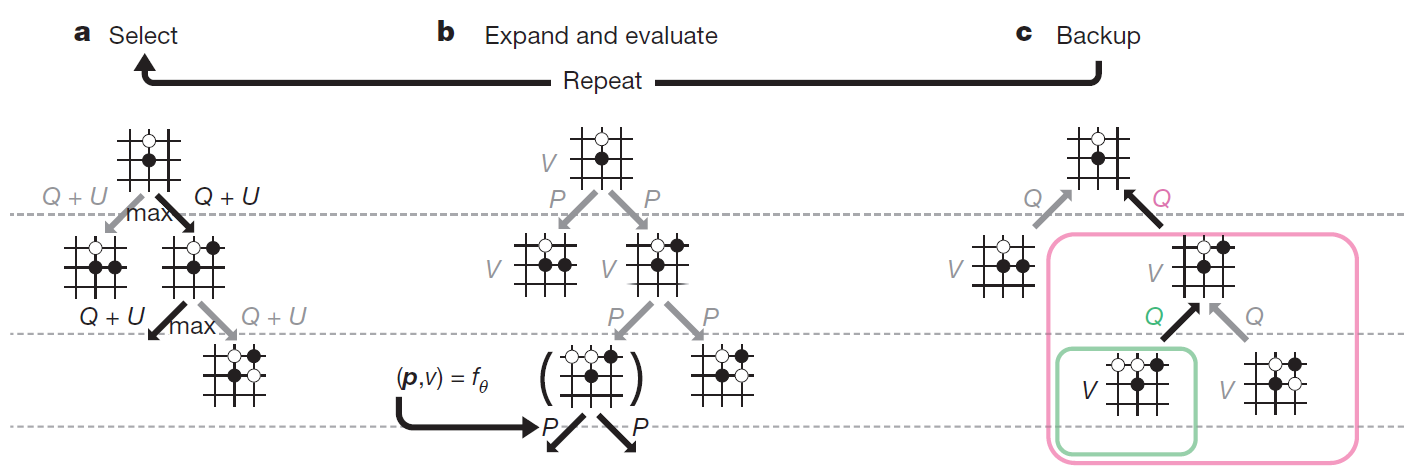
\includegraphics[width=\textwidth]{../img/AG0-paper/MCTS-1.png}
      \end{center}
    \end{frame}

    \begin{frame}{AG0: Monte Carlo Tree Search (2/2)}
      \begin{center}
        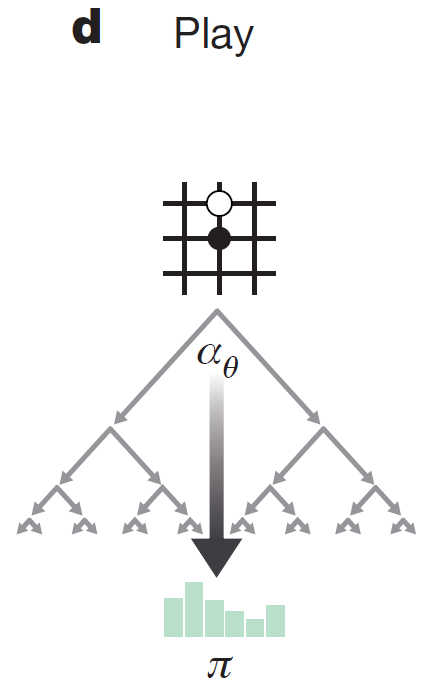
\includegraphics[height=.85\textheight]{../img/AG0-paper/MCTS-2.png}
      \end{center}
    \end{frame}

    \begin{frame}{AG0: Self-Play Reinforcement Learning -- Review}
      \begin{center}
        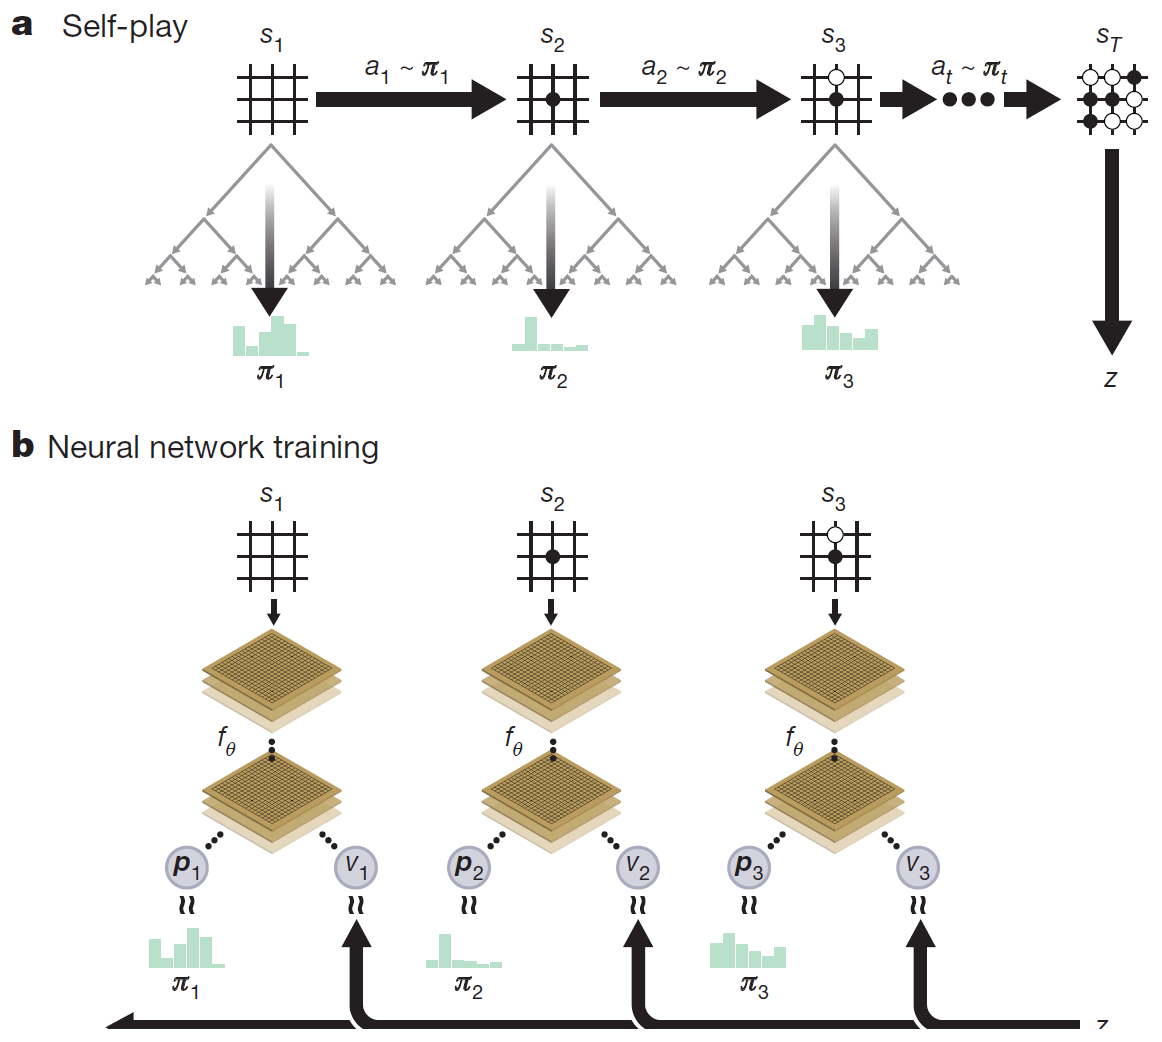
\includegraphics[height=.9\textheight]{../img/AG0-paper/self-play-RL-in-AG0.png}
      \end{center}
    \end{frame}

    \begin{frame}{AG0: Elo Rating over Training Time (RL vs. SL)}
      \begin{center}
        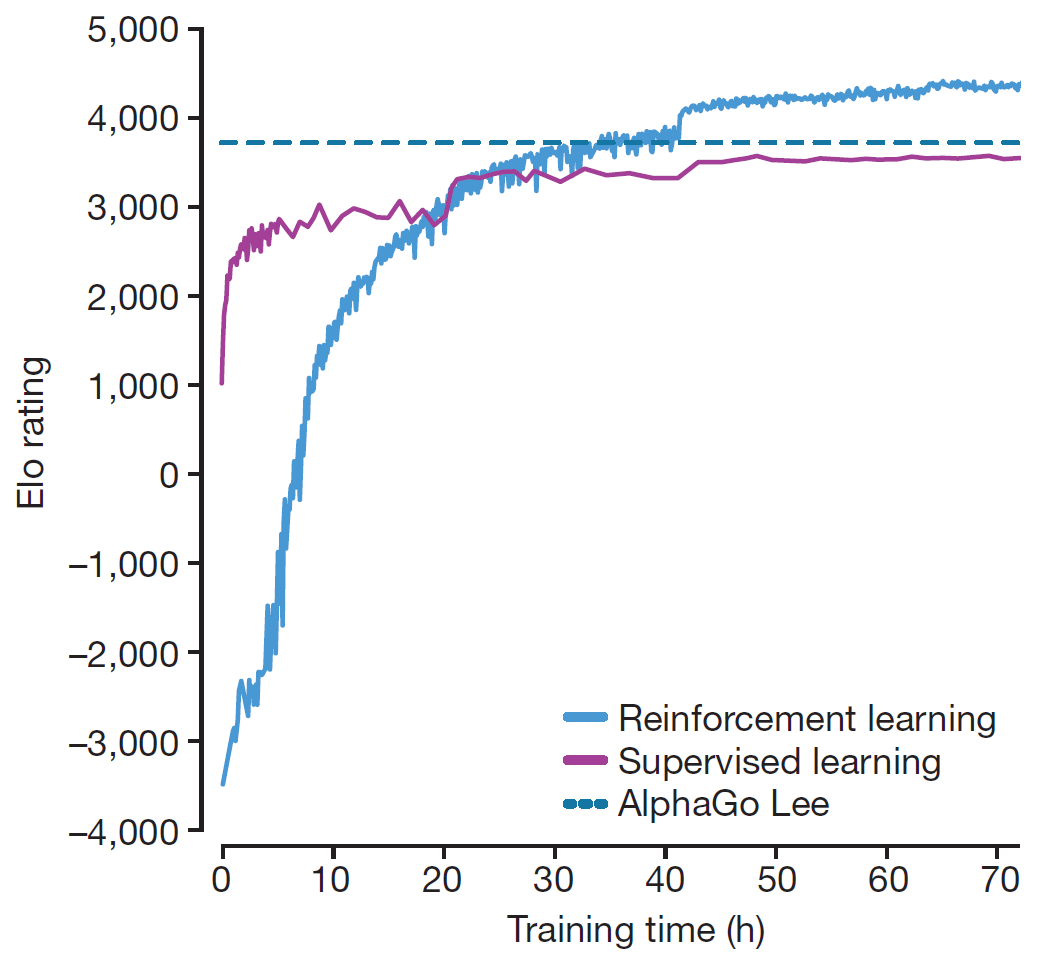
\includegraphics[height=.9\textheight]{../img/AG0-paper/training-time-vs-elo.png}
      \end{center}
    \end{frame}

    \begin{frame}{AG0: Elo Rating over Training Time (AG0 with 40 blocks)}
      \begin{center}
        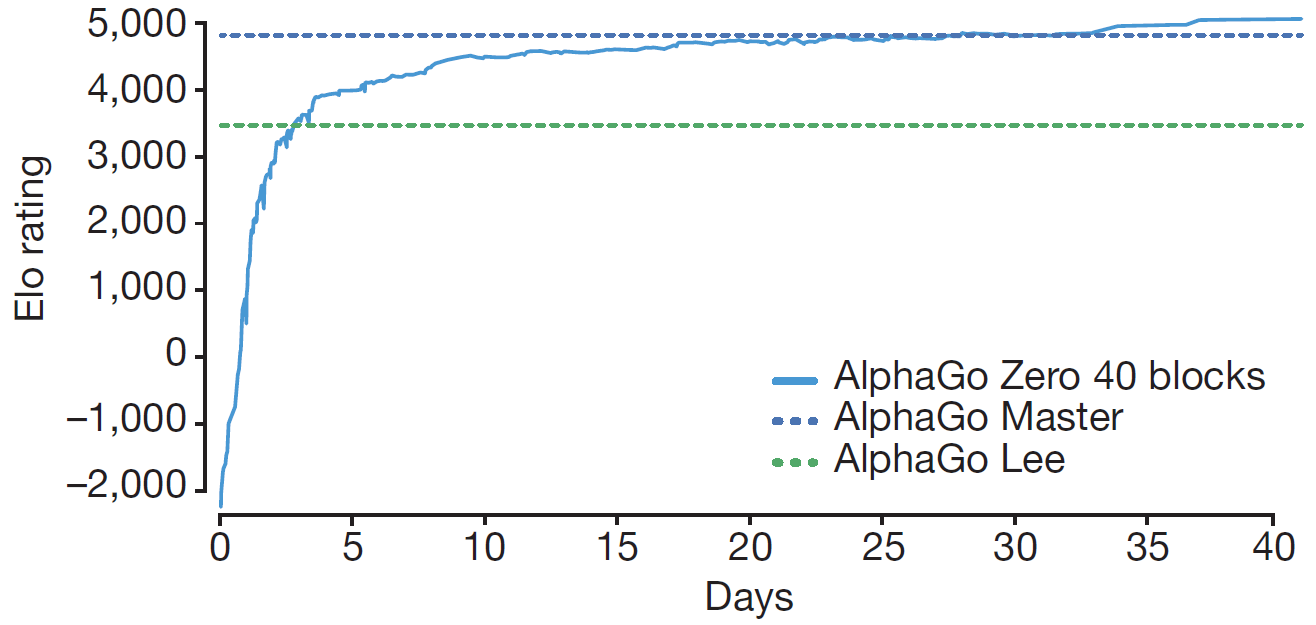
\includegraphics[width=\textwidth]{../img/AG0-paper/AG0-40-elo-vs-training-days.png}
      \end{center}
    \end{frame}

    \begin{frame}{AG0: Tournament between AI Go Programs}
      \begin{center}
        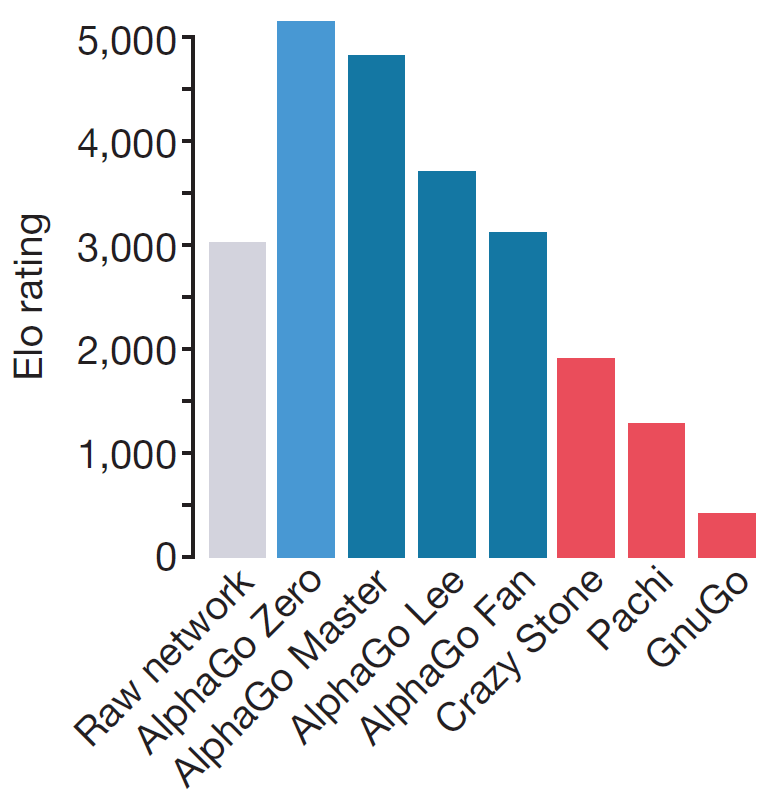
\includegraphics[height=.9\textheight]{../img/AG0-paper/elo-from-tournament.png}
      \end{center}
    \end{frame}

    \begin{frame}{AG0: Discovered Joseki (Corner Sequences)}
      \begin{center}
        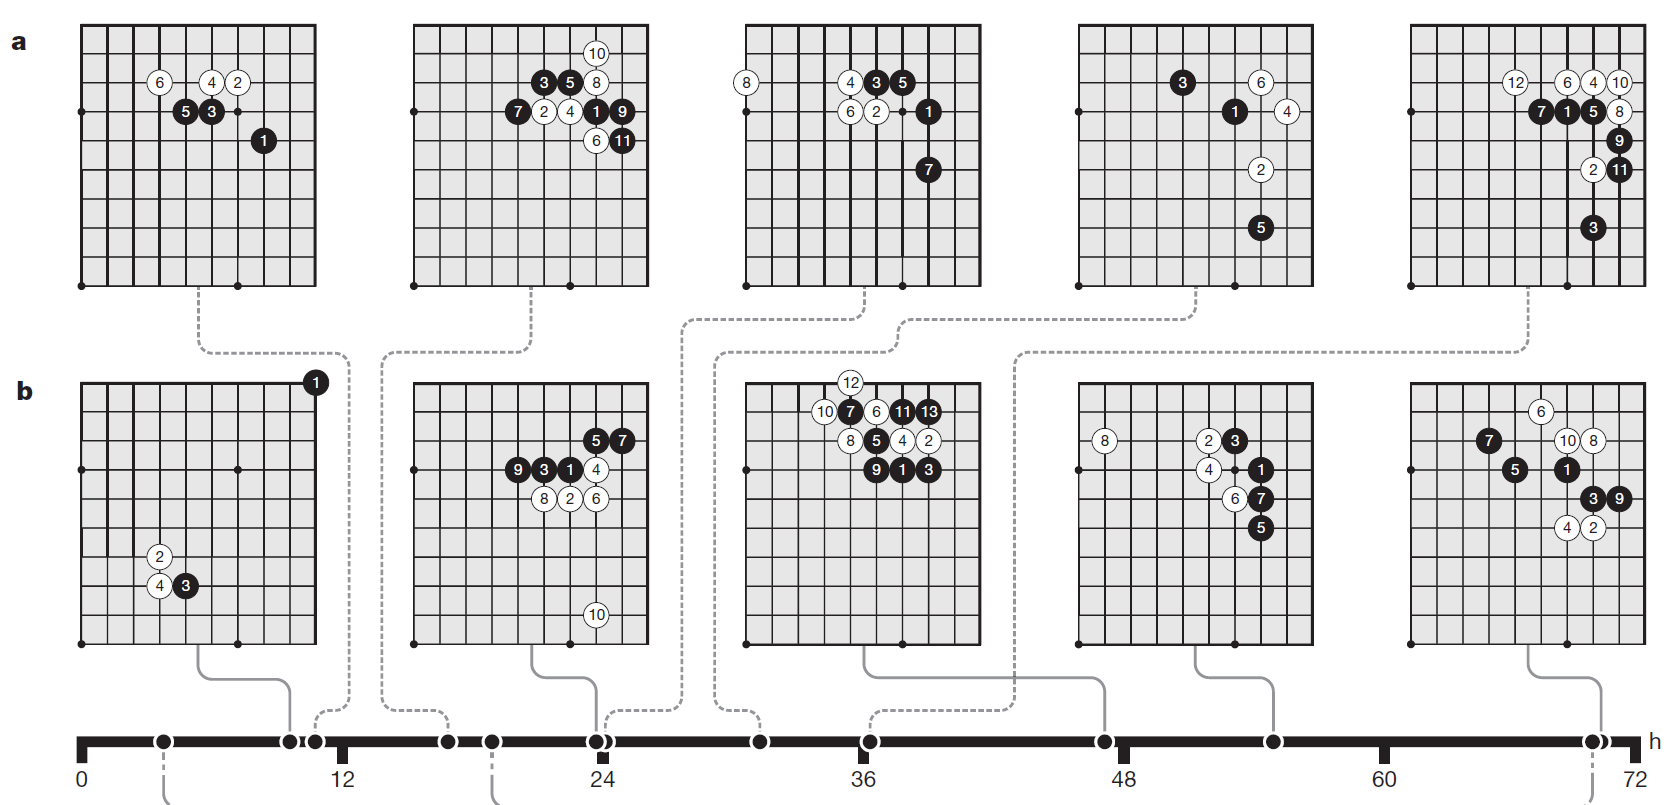
\includegraphics[width=\textwidth]{../img/AG0-paper/discovered-openings.png}
      \end{center}
      \pause

      \begin{description}[<+- | alert@+>]
        \item[a] five human \textit{joseki}
        \item[b] five novel \textit{joseki} variants eventually preferred by AG0
      \end{description}
    \end{frame}

    \begin{frame}{AG0: Discovered Playing Styles}
      \begin{center}
        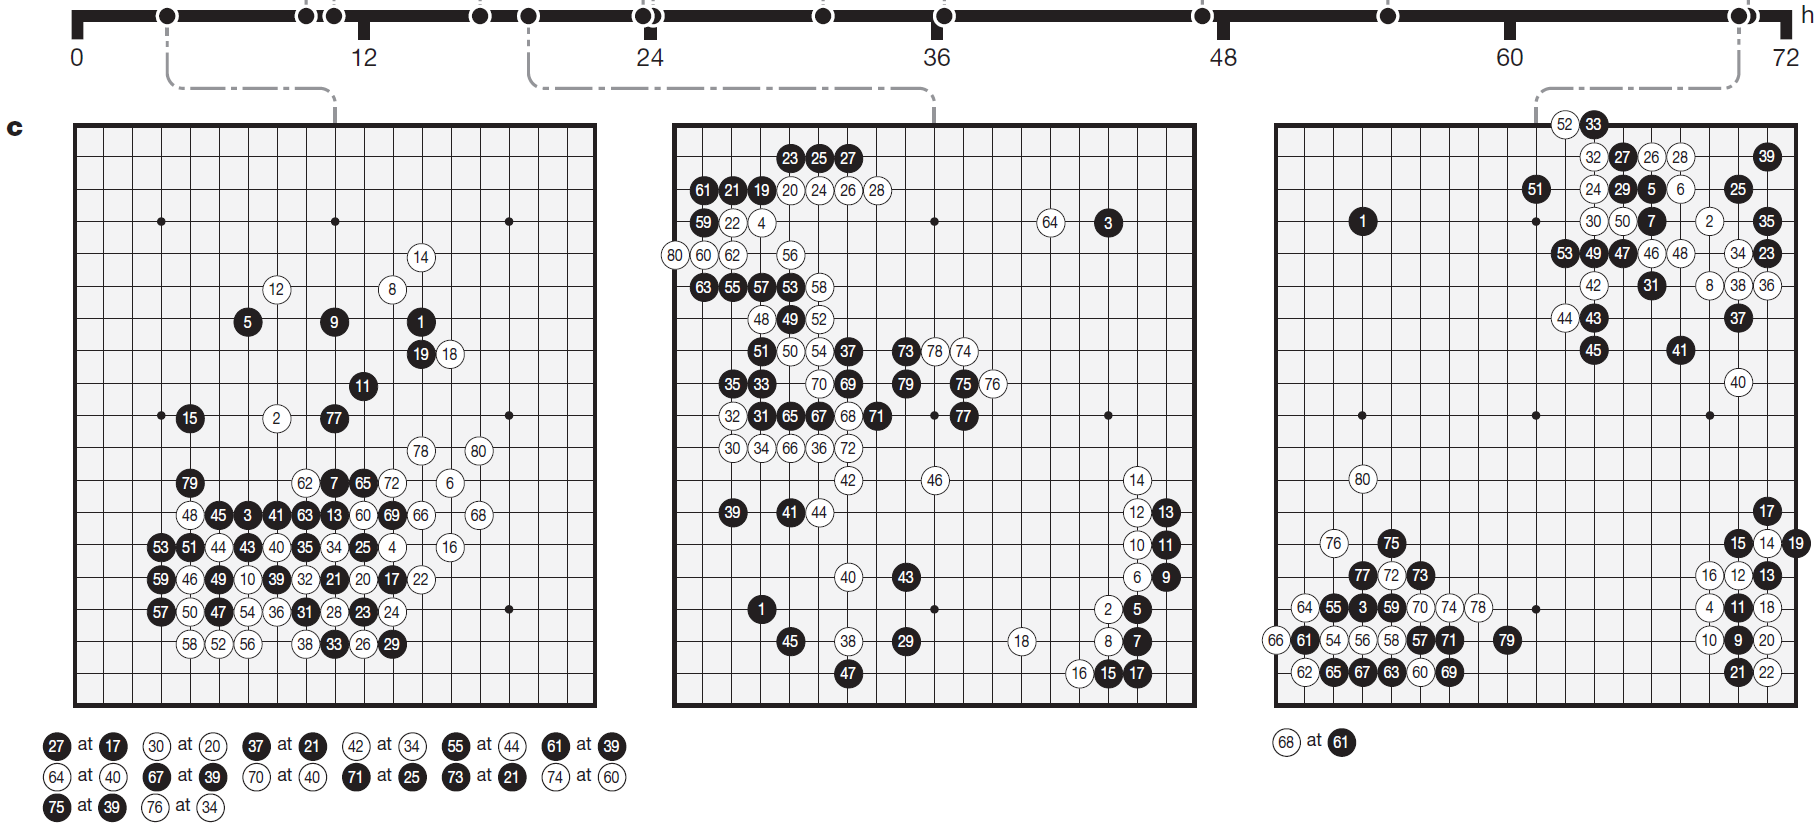
\includegraphics[width=\textwidth]{../img/AG0-paper/playing-styles-discovered-in-time.png}
      \end{center}
      \pause

      \vskip -.5cm
      \begin{description}[<+- | alert@+>]
        \item[at 3 h] greedy capture of stones
        \item[at 19 h] the fundamentals of Go concepts (life-and-death, influence, territory...)
        \item[at 70 h] remarkably balanced game (multiple battles, complicated \textit{ko} fight, a~half-point win for white...)
      \end{description}
    \end{frame}
  }

%%%%%%%%%%%%%%%%%%%%%%%%%%%%%%%%%%%%%%%%%%%%%%%%%%%%%%%%%%%%%%%%%%%%%%%%%%%%%%%%

  \section{AlphaZero}
  {
    \usebackgroundtemplate{
      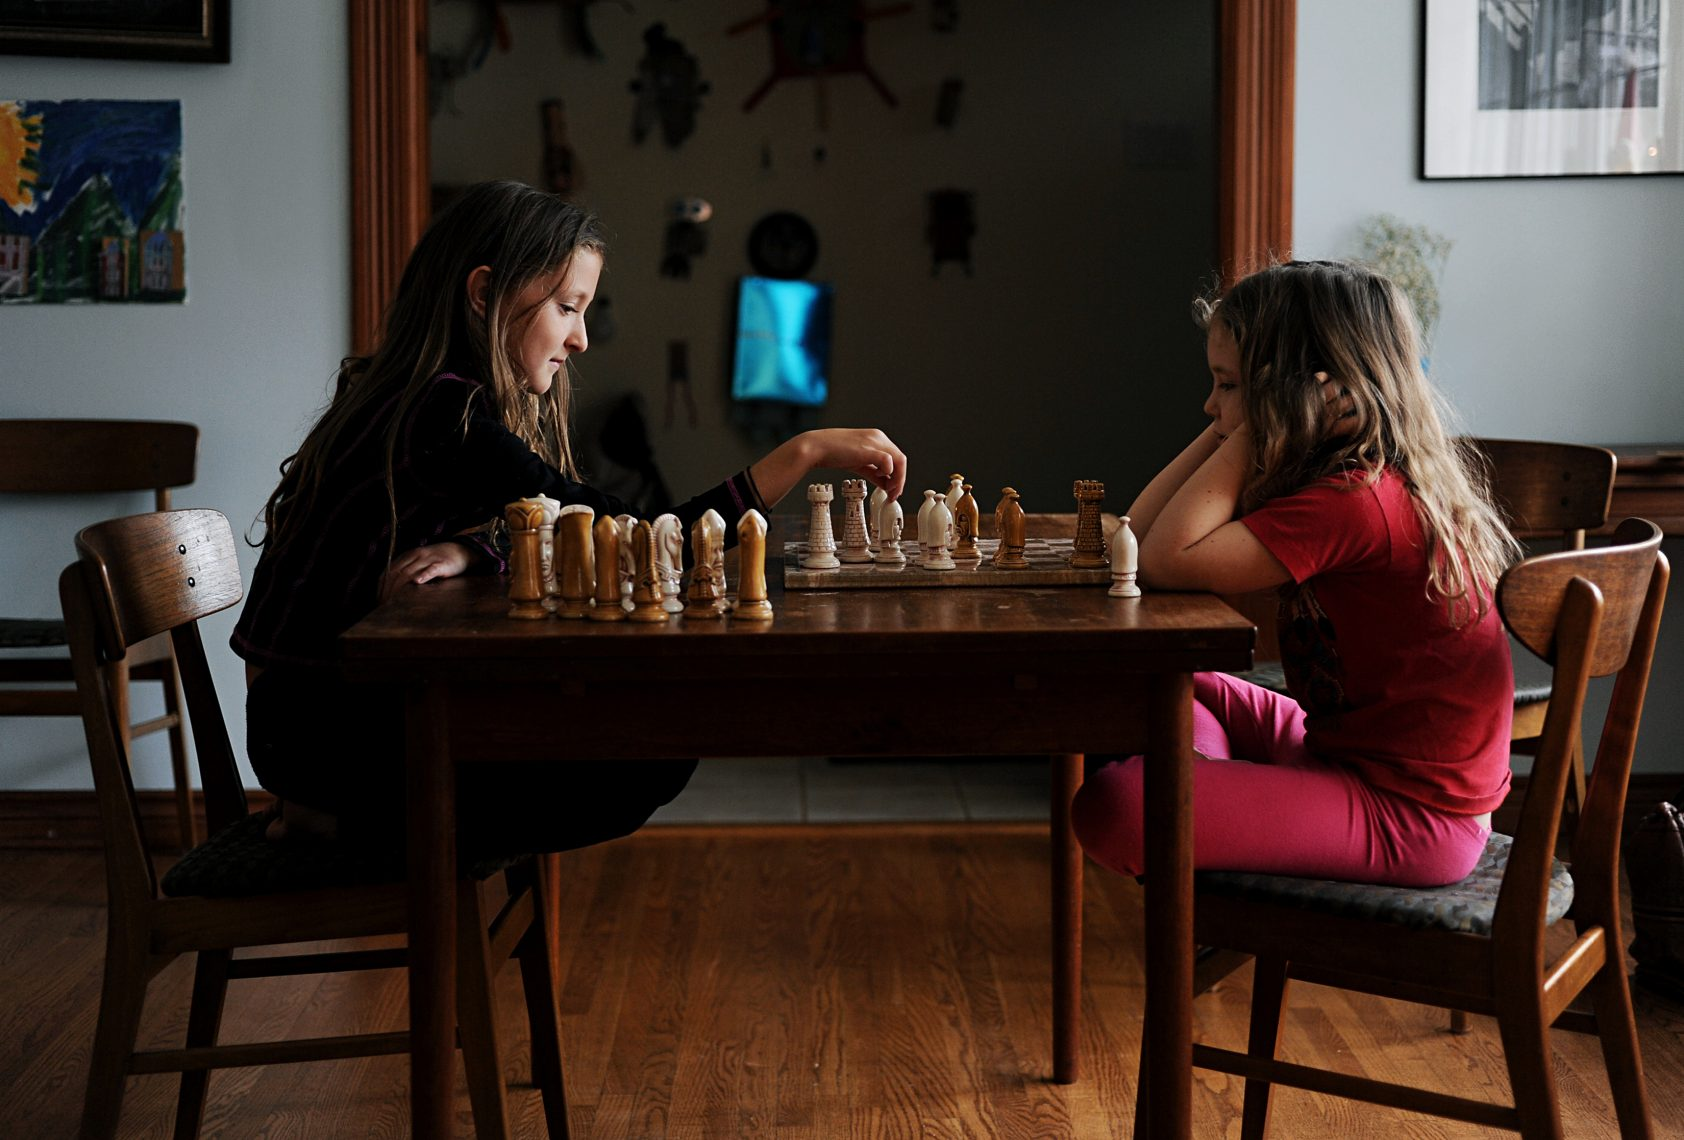
\includegraphics[height=\paperheight]{../img/girls_playing_chess.jpg}
    }
    \begin{frame}[standout]
      \pause
      \vskip .5\textheight

      \epigraph{
        \tiny
        To watch such a~strong programme like Stockfish, against whom most top players would be happy to win even one game out of a~hundred, being completely taken apart is certainly definitive.
      }{Viswanathan Anand}

      \pause
      \epigraph{
        \tiny
        It’s like chess from another dimension.
      }{Demis Hassabis}
    \end{frame}
  }

  {
    \setbeamertemplate{frame footer}{[\cite{Silver2017AlphaZero}]}

    \begin{frame}{AlphaZero: Differences Compared to AlphaGo Zero}
      AlphaGo Zero $\times$ \alert{AlphaZero}:
      \pause
      \begin{itemize}[<+->]
        \item binary outcome (win / loss) $\times$ \alert{expected outcome (including draws or potentially other outcomes)}
        \item board positions transformed before passing to neural networks (by randomly selected rotation or reflection) $\times$ \alert{no data augmentation}
        \item games generated by the best player from previous iterations (margin of 55~\%) $\times$ \alert{continual update using the latest parameters (without the evaluation and selection steps)}
        \item hyper-parameters tuned by Bayesian optimisation $\times$ \alert{reused the same hyper-parameters without game-specific tuning}
      \end{itemize}
    \end{frame}

    \begin{frame}{AlphaZero: Openings Discovered by the Self-Play (1/2)}
      \begin{center}
        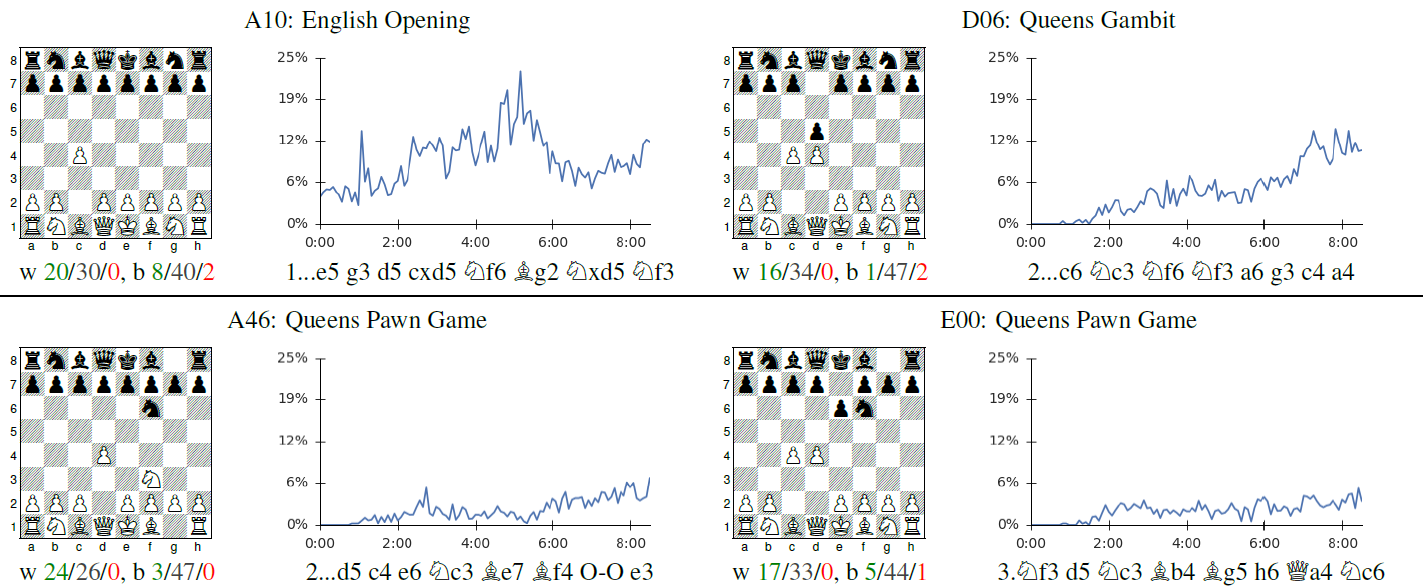
\includegraphics[width=\textwidth]{../img/AlphaZero-paper/openings-1.png}
      \end{center}
    \end{frame}

    \begin{frame}{AlphaZero: Openings Discovered by the Self-Play (2/2)}
      \begin{center}
        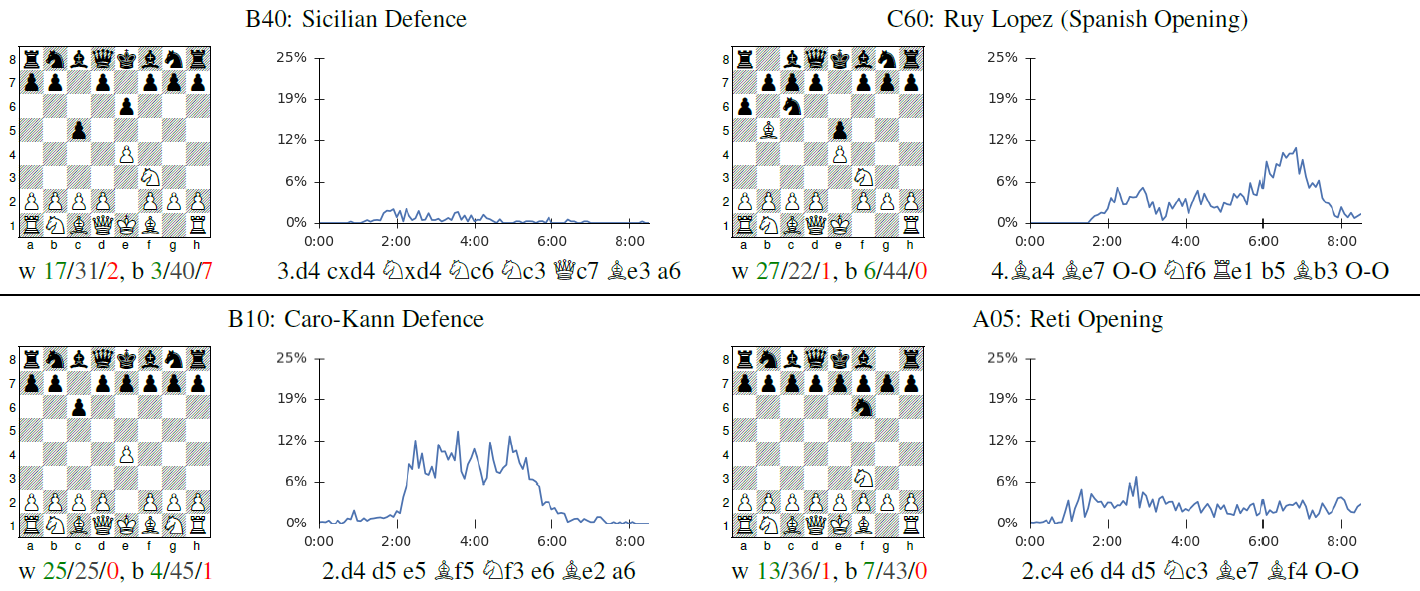
\includegraphics[width=\textwidth]{../img/AlphaZero-paper/openings-2.png}
      \end{center}
    \end{frame}

    \begin{frame}{AlphaZero: Elo Rating over Training Time}
      \begin{center}
        \pause
        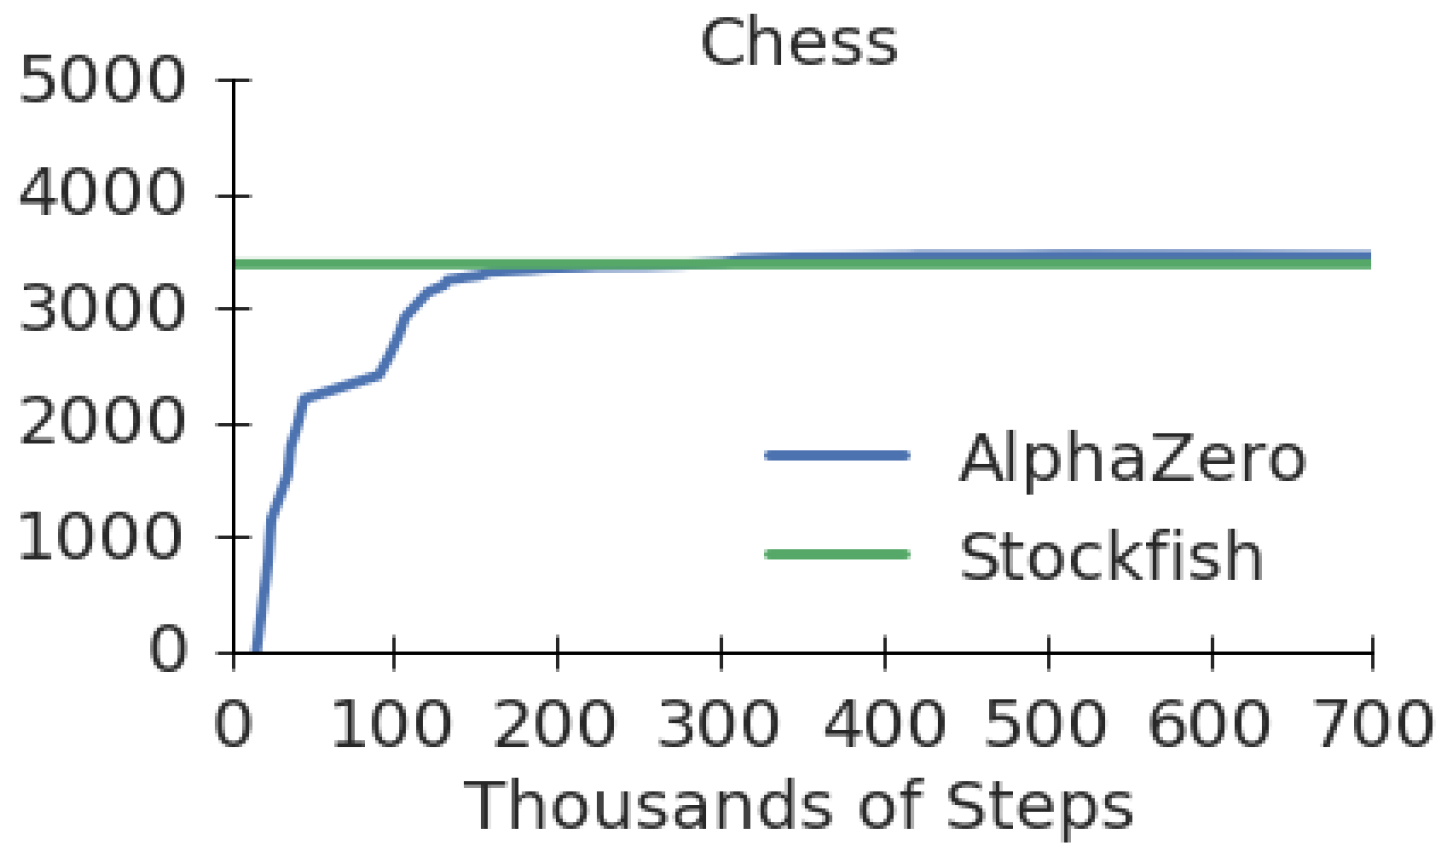
\includegraphics[width=.5\textwidth]{../img/AlphaZero-paper/elo-vs-training-chess.png}
        \pause
        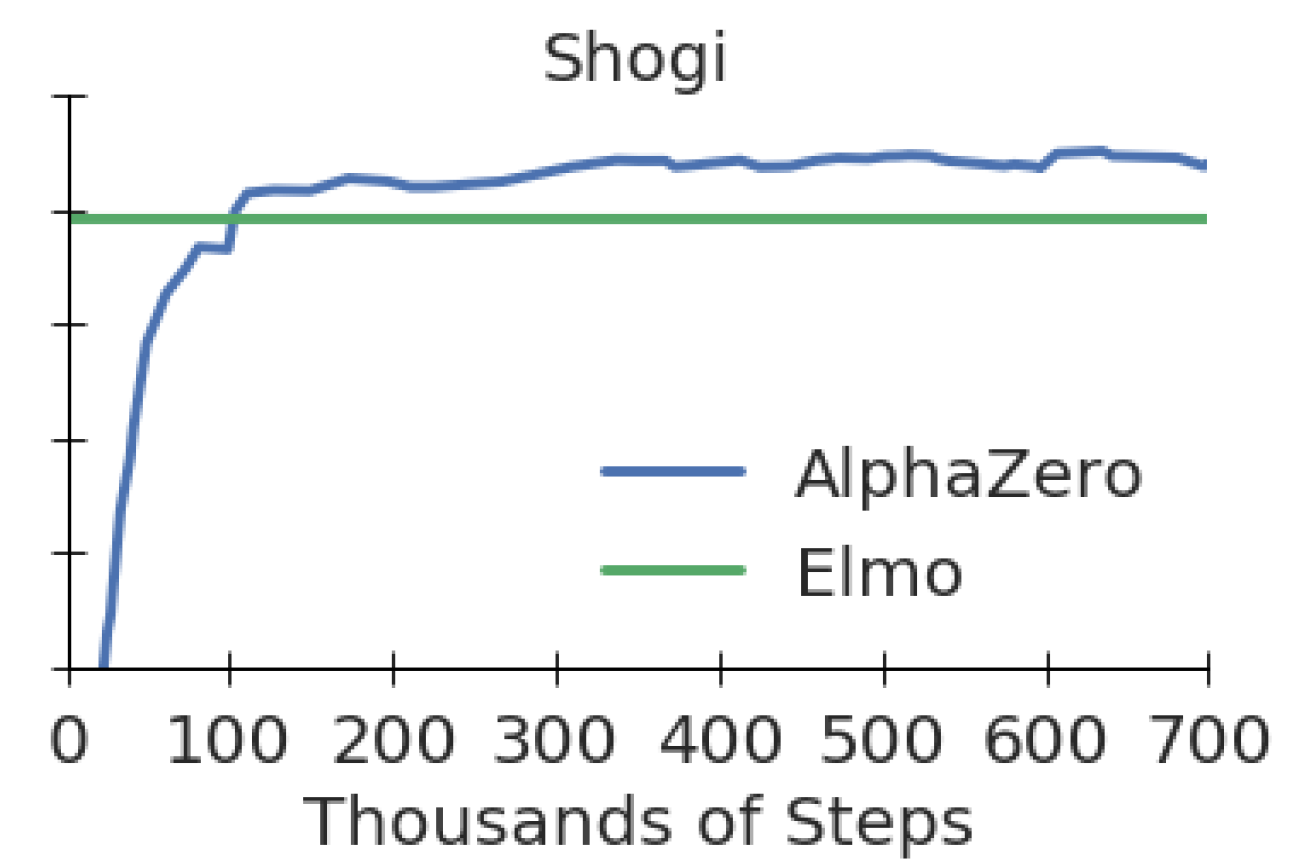
\includegraphics[width=.5\textwidth]{../img/AlphaZero-paper/elo-vs-training-shogi.png}

        \pause
        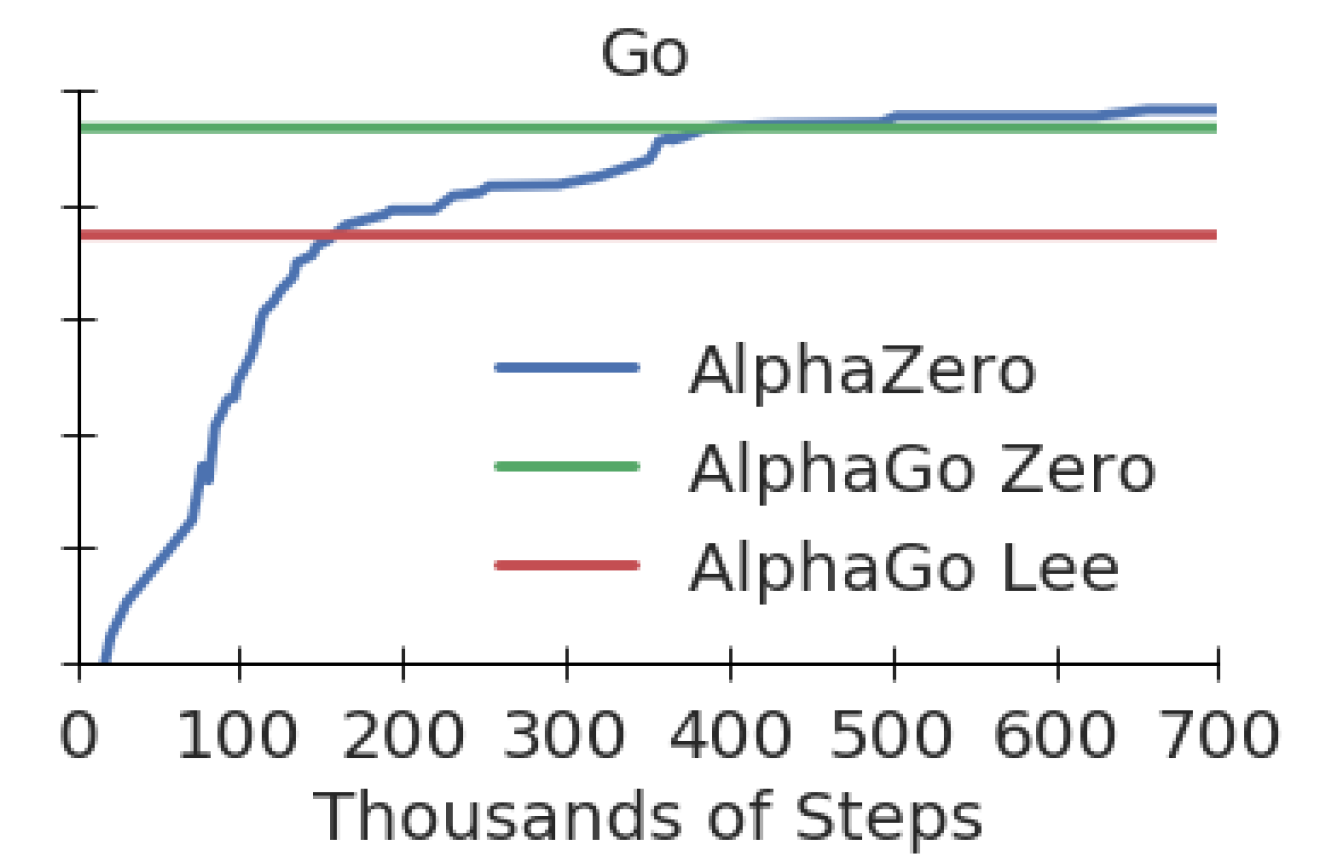
\includegraphics[height=.4\textheight]{../img/AlphaZero-paper/elo-vs-training-go.png}
      \end{center}
    \end{frame}

    \begin{frame}{AlphaZero: Tournament between AI Programs}
      \begin{center}
        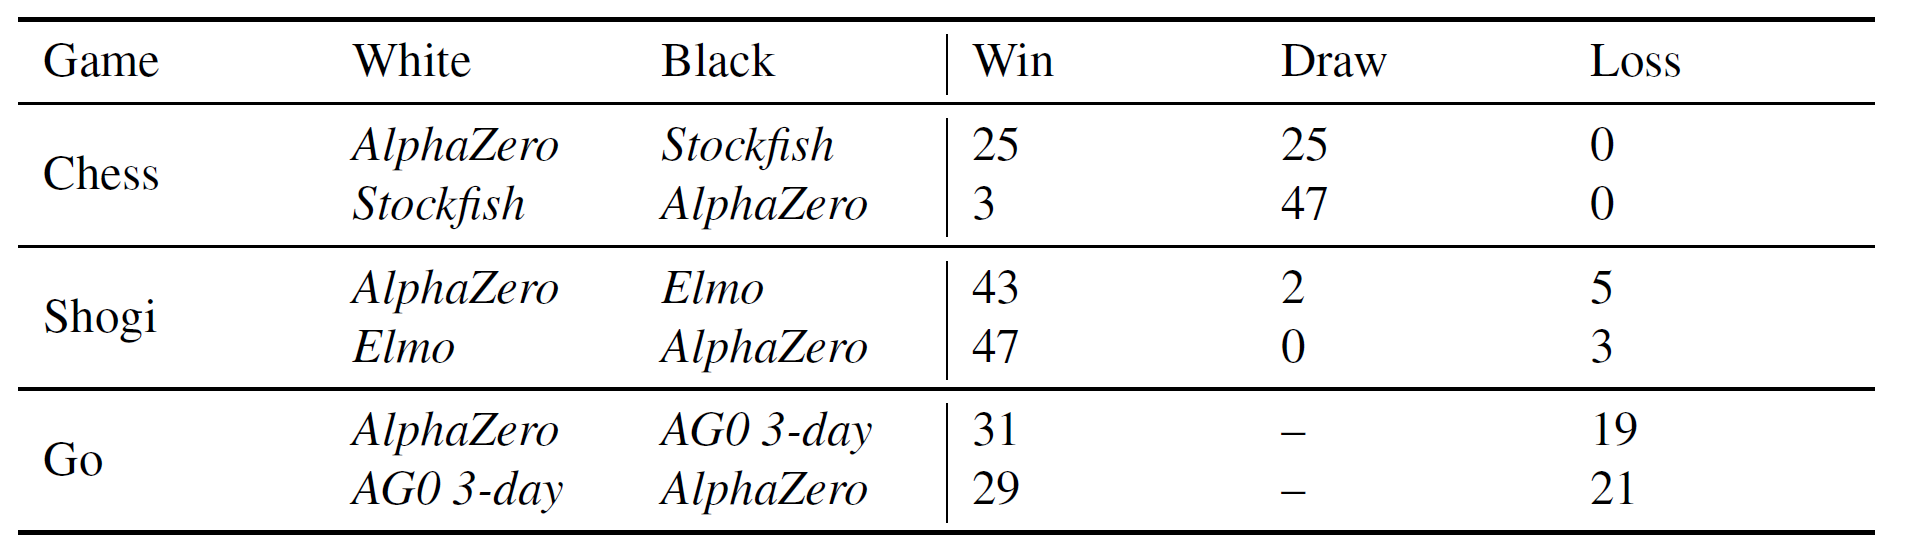
\includegraphics[width=\textwidth]{../img/AlphaZero-paper/tournament-evaluation.png}
      \end{center}

      {\tiny (Values are given from AlphaZero's point of~view.)}
    \end{frame}

    \begin{frame}{AlphaZero: Statistics of Training}
      \begin{center}
        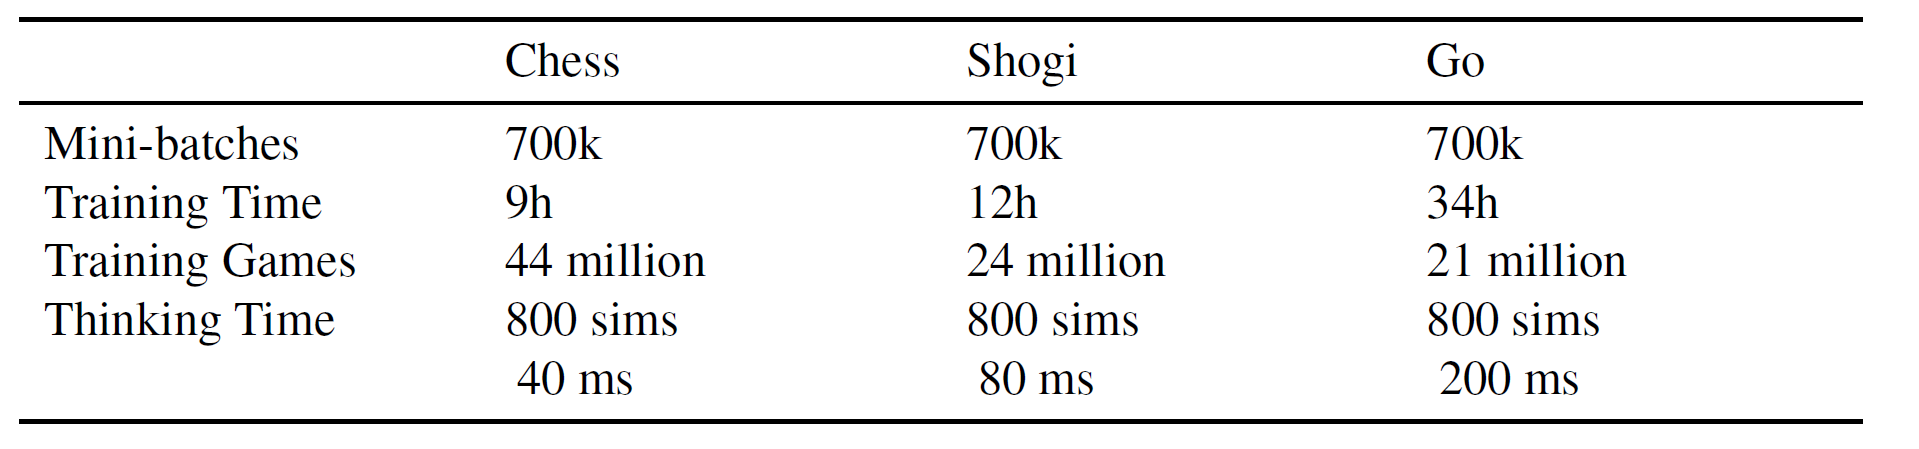
\includegraphics[width=\textwidth]{../img/AlphaZero-paper/statistics-of-AlphaZero-training.png}
      \end{center}
    \end{frame}

    \begin{frame}{AlphaZero: Evaluation Speeds}
      \begin{center}
        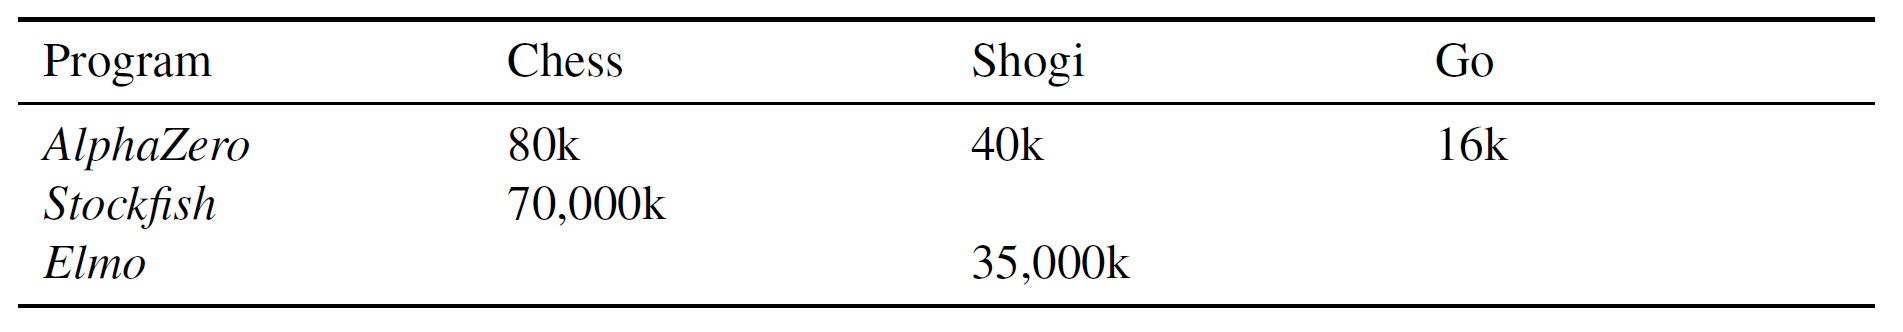
\includegraphics[width=\textwidth]{../img/AlphaZero-paper/evaluation-speed-of-AlphaZero.png}
      \end{center}
    \end{frame}
  }

  \section{Conclusion}

  {
    \setbeamertemplate{frame footer}{[\cite{Silver2017AlphaZero}]}
    \begin{frame}{Difficulties of~Go}
      \begin{itemize}[<+- | alert@+>]
        \item challenging decision-making
        \item intractable search space
        \item complex optimal solution

          {\tiny It appears infeasible to directly approximate using a~policy or value function!}
      \end{itemize}
    \end{frame}

    \begin{frame}{AlphaZero: Summary}
      \begin{itemize}[<+- | alert@+>]
        \item Monte Carlo tree search
        \item effective move selection and position evaluation 
          \begin{itemize}[<+- | alert@+>]
            \item through deep convolutional neural networks
            \item trained by new self-play reinforcement learning algorithm
          \end{itemize}
        \item new search algorithm combining
          \begin{itemize}[<+- | alert@+>]
            \item evaluation by a~single neural network
            \item Monte Carlo tree search
          \end{itemize}
        \item more efficient when compared to previous AlphaGo versions
          \begin{itemize}[<+- | alert@+>]
            \item single machine
            \item 4 TPUs
            \item hours rather than months of~training time
          \end{itemize}
      \end{itemize}
    \end{frame}

    \begin{frame}{Novel approach}
      \pause
      During the matches (against Stockfish and Elmo), AlphaZero evaluated \alert{thousands of~times fewer} positions than Deep~Blue against Kasparov.
      \pause

      It compensated this by:
      \begin{itemize}[<+->]
        \item selecting those positions \alert{more intelligently} (the neural network)
        \item evaluating them \alert{more precisely} (the same neural network)
      \end{itemize}
      \pause

      Deep~Blue relied on a~handcrafted evaluation function.
      \pause

      AlphaZero was trained \alert{tabula rasa} from self-play.
      It used \alert{general-purpose} learning.
      \pause

      This approach is not specific to the game of~Go.
      The algorithm can be used \alert{for much wider class} of~AI problems!
    \end{frame}
  }

  \begin{frame}[standout]
    \begin{center}
      Thank you!

      Questions?
    \end{center}
  \end{frame}

  \begin{frame}[standout]
    Backup Slides
  \end{frame}

%%%%%%%%%%%%%%%%%%%%%%%%%%%%%%%%%%%%%%%%%%%%%%%%%%%%%%%%%%%%%%%%%%%%%%%%%%%%%%%%

  \appendix
  \begin{frame}[standout]
    Backup Slides
  \end{frame}

  {
    \setbeamertemplate{frame footer}{[\cite{Silver2017AlphaZero}]}

    \begin{frame}{Input Features of AlphaZero's Neural Networks}
      \begin{center}
        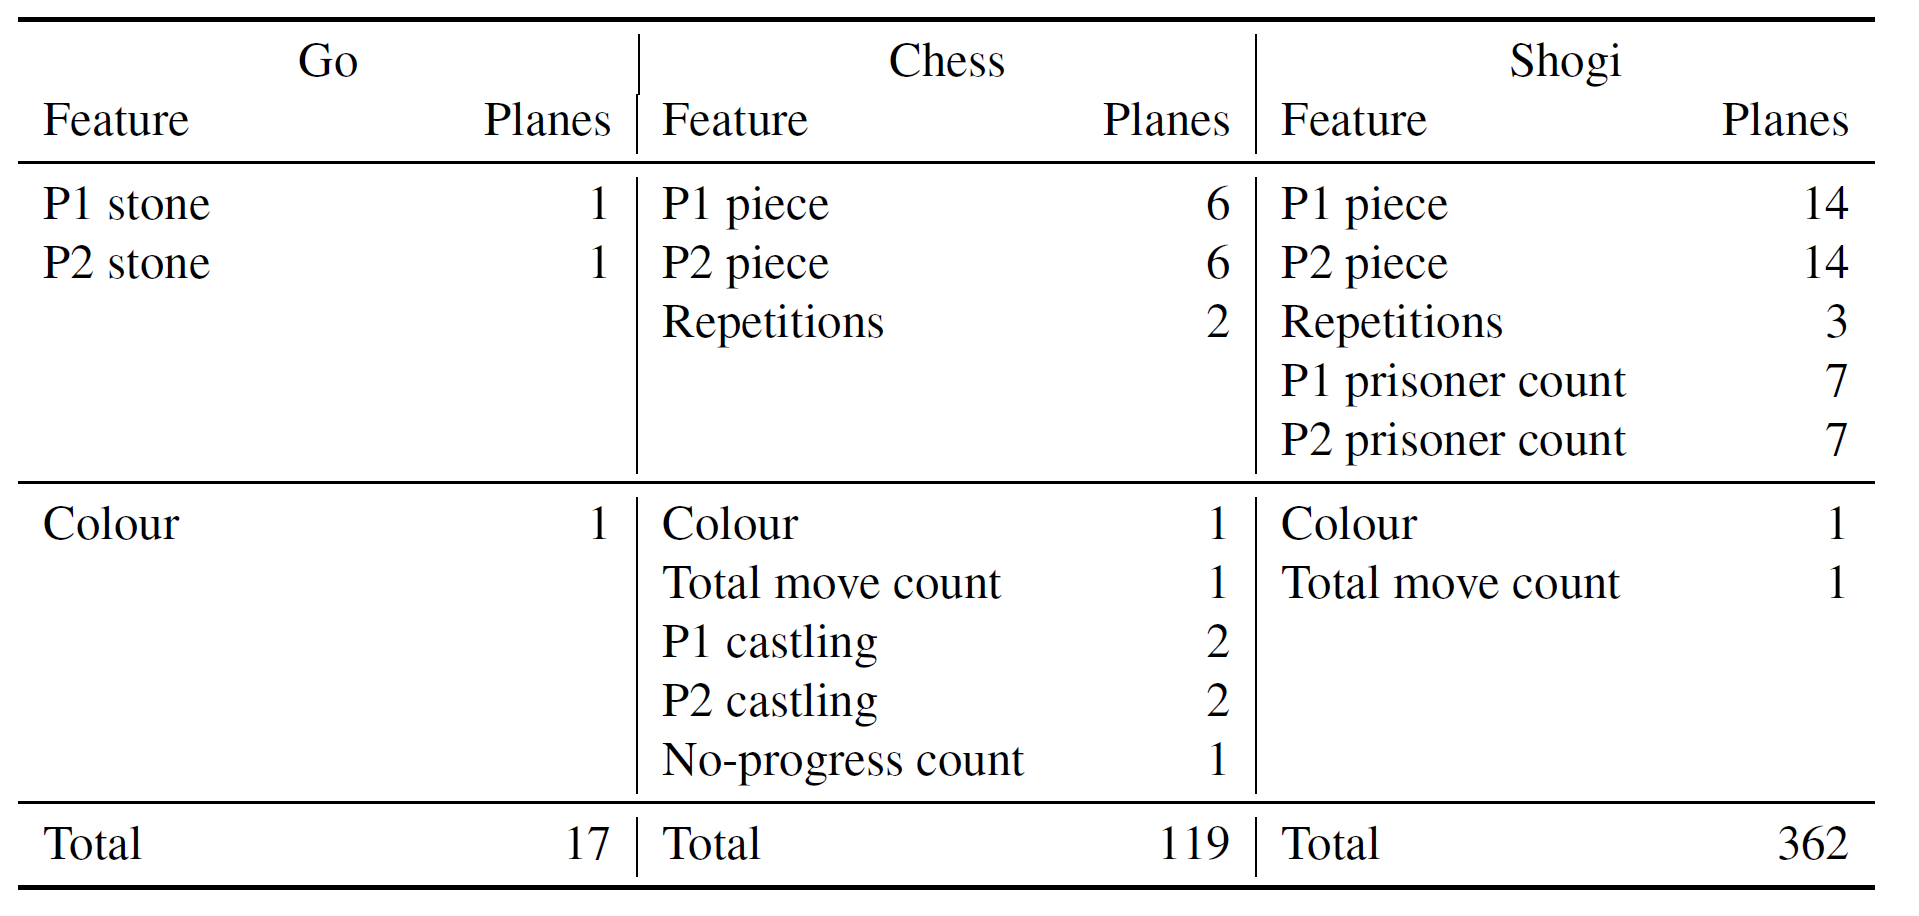
\includegraphics[width=\textwidth]{../img/AlphaZero-paper/input-features.png}
      \end{center}
    \end{frame}

    \begin{frame}{Scalability When Compared to Other Programs}
      \begin{center}
        \pause
        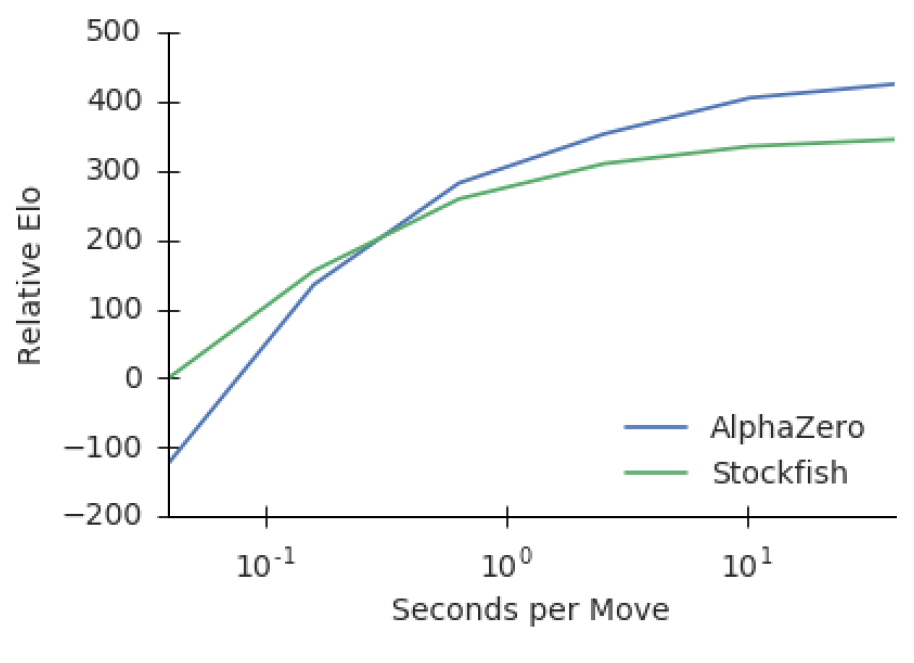
\includegraphics[height=.45\textheight]{../img/AlphaZero-paper/scalability-against-stockfish.png}

        \pause
        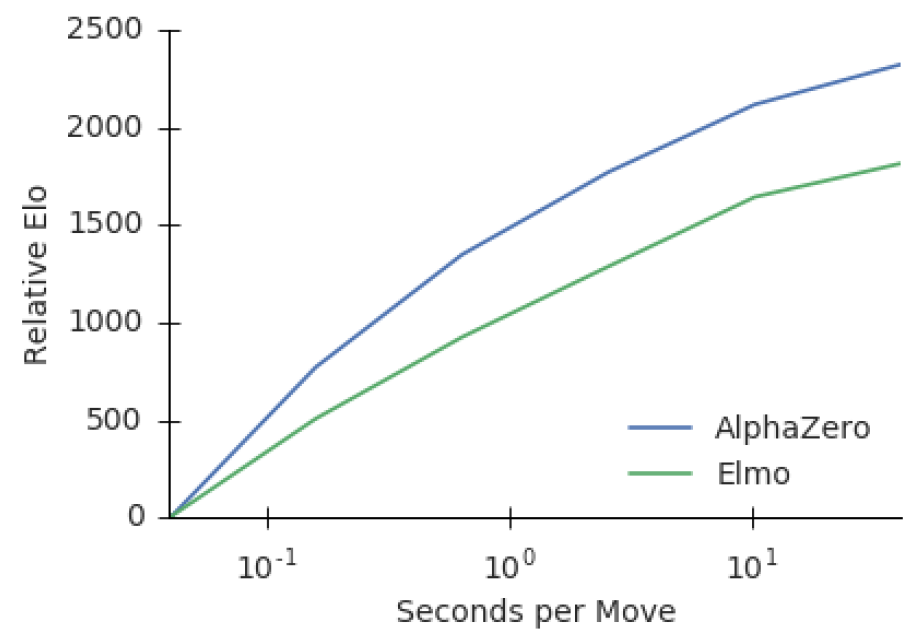
\includegraphics[height=.45\textheight]{../img/AlphaZero-paper/scalability-against-elmo.png}
      \end{center}
    \end{frame}
  }

  \begin{frame}[allowframebreaks]{Further Reading}
    \tiny
    AlphaGo:
    \begin{itemize}
      \item \textbf{Google Research Blog} \url{http://googleresearch.blogspot.cz/2016/01/alphago-mastering-ancient-game-of-go.html}
      \item an article in \textbf{Nature} \url{http://www.nature.com/news/google-ai-algorithm-masters-ancient-game-of-go-1.19234}
      \item a \textbf{reddit} article claiming that AlphaGo is even stronger than it appears to be: \\
        ``AlphaGo would rather win by less points, but with higher probability.'' \\
        \url{https://www.reddit.com/r/baduk/comments/49y17z/the_true_strength_of_alphago/}
      \item a~video of~how AlphaGo works (put in layman's terms) \url{https://youtu.be/qWcfiPi9gUU}
    \end{itemize}

    Articles by Google DeepMind:
    \begin{itemize}
      \item \textbf{Atari player}: a DeepRL system which combines Deep Neural Networks with Reinforcement Learning (\cite{Mnih2015human})
      \item \textbf{Neural Turing Machines} (\cite{Graves2014neural})
    \end{itemize}

    Artificial Intelligence:
    \begin{itemize}
      \item \textbf{Artificial Intelligence course at MIT} \url{http://ocw.mit.edu/courses/electrical-engineering-and-computer-science/6-034-artificial-intelligence-fall-2010/index.htm}
      \item \textbf{Introduction to Artificial Intelligence at Udacity} \url{https://www.udacity.com/course/intro-to-artificial-intelligence--cs271}
      \item \textbf{General Game Playing course} \url{https://www.coursera.org/course/ggp}
      \item \textbf{Singularity} \url{http://waitbutwhy.com/2015/01/artificial-intelligence-revolution-1.html} + Part 2
      \item \textbf{The Singularity Is Near} (\cite{Kurzweil2005singularity})
    \end{itemize}

    Combinatorial Game Theory (founded by John H. Conway to study endgames in Go):
    \begin{itemize}
      \item \textbf{Combinatorial Game Theory course} \url{https://www.coursera.org/learn/combinatorial-game-theory}
      \item On Numbers and Games (\cite{Conway1976number})
      \item Computer Go as a sum of local games: an application of combinatorial game theory (\cite{Muller1995computer})
    \end{itemize}

    Chess:
    \begin{itemize}
      \item \textbf{Deep Blue beats G. Kasparov in 1997} \url{https://youtu.be/NJarxpYyoFI}
    \end{itemize}

    Machine Learning:
    \begin{itemize}
      \item \textbf{Machine Learning course} \url{https://youtu.be/hPKJBXkyTK://www.coursera.org/learn/machine-learning/}
      \item \textbf{Reinforcement Learning} \url{http://reinforcementlearning.ai-depot.com/}
      \item \textbf{Deep Learning} (\cite{Lecun2015deep})
      \item \textbf{Deep Learning course} \url{https://www.udacity.com/course/deep-learning--ud730}
      \item \textbf{Two Minute Papers} \url{https://www.youtube.com/user/keeroyz}
      \item \textbf{Applications of Deep Learning} \url{https://youtu.be/hPKJBXkyTKM}
    \end{itemize}

    Neuroscience:
    \begin{itemize}
      \item \url{http://www.brainfacts.org/}
    \end{itemize}
  \end{frame}

  \begin{frame}[allowframebreaks]{References}
    \tiny
    \printbibliography[heading=none]
  \end{frame}

\end{document}
